\chapter{Performance evaluation}
\label{chap:experiments}

\section{Design of the experiments}

To perform a complete evaluation of the LoRaWAN technology a preliminary analysis was done in order to discover all the configurable parameters. As result of this operation the following settings were taken into account:
\begin{itemize}
\item \emph{Environment}: rural and urban;
\item \emph{Data Rate}: the combination of spreading factor and bandwidth defines the rate at which data is transmitted;
\item \emph{Coding Rate}: the level of forward error correction;
\item \emph{Distance}: the relative distance between end-device and gateway;
\item \emph{Packet length};
\item \emph{Transmission power};
\end{itemize}
Two relevant evaluation metrics have been identified: the  \emph{Packet Error Rate} and \emph{Power Consumption}. Due to the limitations of the available hardware, only the \emph{Packet Error Rate} has been tested. 


\subsection{Analysis of the parameters}

\subsubsection{Environment}
Since the specification of LoRaWAN reports very different behaviors depending on the environment in which experiments are performed, it has been decided to consider two different scenarios:
\begin{itemize}
\item \emph{Rural environment}: both gateway and end-devices are placed outside buildings, and all measurements are done in not line of sight condition in an area with a low density of buildings and high presence of trees;

\item \emph{Urban environment}: while the gateway is placed outside, the end-devices are placed inside buildings in the center of Pisa.
\end{itemize}


\subsubsection{Data Rate}
% Please add the following required packages to your document preamble:
% \usepackage{booktabs}
\begin{table}[]
\centering
\caption{Data Rates available on Waspmote Pro}
\label{tab:datarates}
\begin{tabular}{@{}ccccc@{}}
\toprule
Data Rate & Code & \begin{tabular}[c]{@{}c@{}}Spreading\\ Factor\end{tabular} & \begin{tabular}[c]{@{}c@{}}Bandwith\\ (kHz)\end{tabular} & \begin{tabular}[c]{@{}c@{}}Speed\\ (bit/s)\end{tabular} \\ \midrule
SF7BW125  & 5    & 7                                                          & 125                                                      & 5470                                                    \\
SF8BW125  & 4    & 8                                                          & 125                                                      & 3125                                                    \\
SF9BW125  & 3    & 9                                                          & 125                                                      & 1760                                                    \\
SF10BW125 & 2    & 10                                                         & 125                                                      & 980                                                     \\
SF11BW125 & 1    & 11                                                         & 125                                                      & 440                                                     \\
SF12BW125 & 0    & 12                                                         & 125                                                      & 250                                                     \\ \bottomrule
\end{tabular}
\end{table}


The rate at which data is transmitted is defined by the combination of spreading factor and bandwidth; the spreading factor is defined as:
\begin{equation}
\label{eq:sf}
\mbox{Spreading Factor} = \frac{\mbox{Chip Rate}}{\mbox{Symbol Rate}}
\end{equation}
where the chip rate is physical available bandwidth, and the symbol rate represents the actual data rate. So, from this equation it is possible to deduce that:
\begin{itemize}
\item increasing the spreading factor the resulting bit rate decreases;
\item increasing the bandwidth the resulting bit rate increases;
\end{itemize}
Table \ref{tab:datarates} shows the available data rate in our setup.

\subsubsection{Coding Rate}
The \emph{Coding Rate} is a parameter of the LoRa physical layer which defines the level of \emph{Forward Error Correction} included into the physical frame. In the LoRa terminology it is represented as a fraction: for instance coding rate 4/5 means that the every 4 bits of actual data, 1 extra bit is added, with a total of 5 bits transmitted on the channel. The possible values of coding rate in LoRa are: 4/5, 4/6, 4/7, 4/8.

\subsubsection{Packet length}
Due to the special features of the LoRa modulation, the maximum payload length changes depending on the spreading factor, as reported in table \ref{tab:payloads}

% Please add the following required packages to your document preamble:
% \usepackage{booktabs}
\begin{table}[]
\centering
\caption{Maximum payload lengths}
\label{tab:payloads}
\begin{tabular}{@{}ccc@{}}
\toprule
\begin{tabular}[c]{@{}c@{}}Spreading\\ Factor\end{tabular} & \begin{tabular}[c]{@{}c@{}}Max MACPayload\\ (bytes)\end{tabular} & \begin{tabular}[c]{@{}c@{}}Max FrmPayload\\ (bytes)\end{tabular} \\ \midrule
7                                                          & 230                                                              & 222                                                              \\
8                                                          & 230                                                              & 222                                                              \\
9                                                          & 123                                                              & 115                                                              \\
10                                                         & 59                                                               & 51                                                               \\
11                                                         & 59                                                               & 51                                                               \\
12                                                         & 59                                                               & 51                                                               \\ \bottomrule
\end{tabular}
\end{table}

\subsubsection{Transmission power}
Considering the 863-870 MHz bandwidth, the available motes for the experiments were able to transmit at: 14 dBm, 11 dBm, 8 dBM, 5 dBm and 2 dBm.




\subsection{Experiments setup}
All experiments were performed using the following setup:
\begin{itemize}
\item \emph{Network Server} Custom LoRa network server, written in Java, described in chapter \ref{chap:server}.
\item \emph{Gateway} Ideetron Lorank 8 LoRa gateway.
\item \emph{End-devices} Libelium Waspmote Pro 1.2, programmed with Waspmote APIs 023. \cite{waspmote}
\end{itemize}


\section{Rural experiments}
\label{sec:ruraltest}
\begin{figure}
\centering
\begin{subfigure}{.5\textwidth}
  \centering
  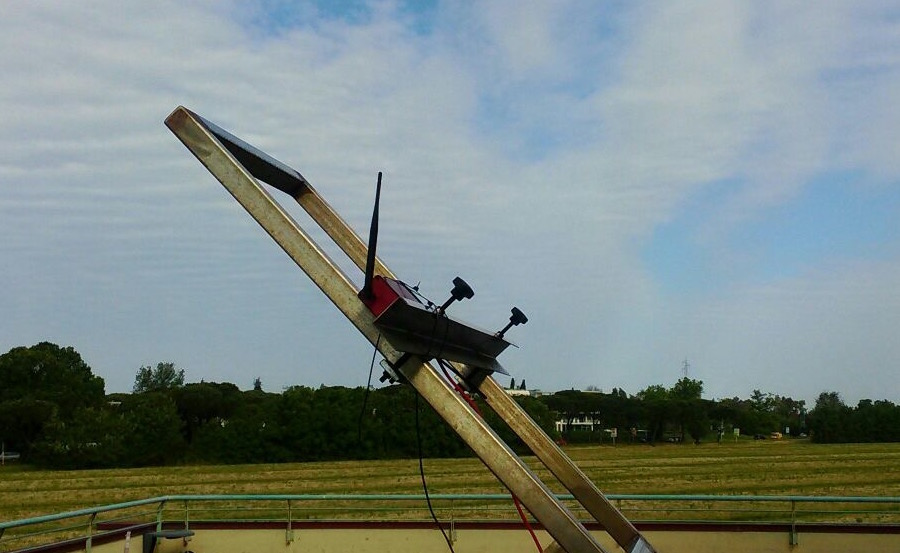
\includegraphics[width=.8\linewidth]{img/gateway}
\end{subfigure}%
\begin{subfigure}{.5\textwidth}
  \centering
  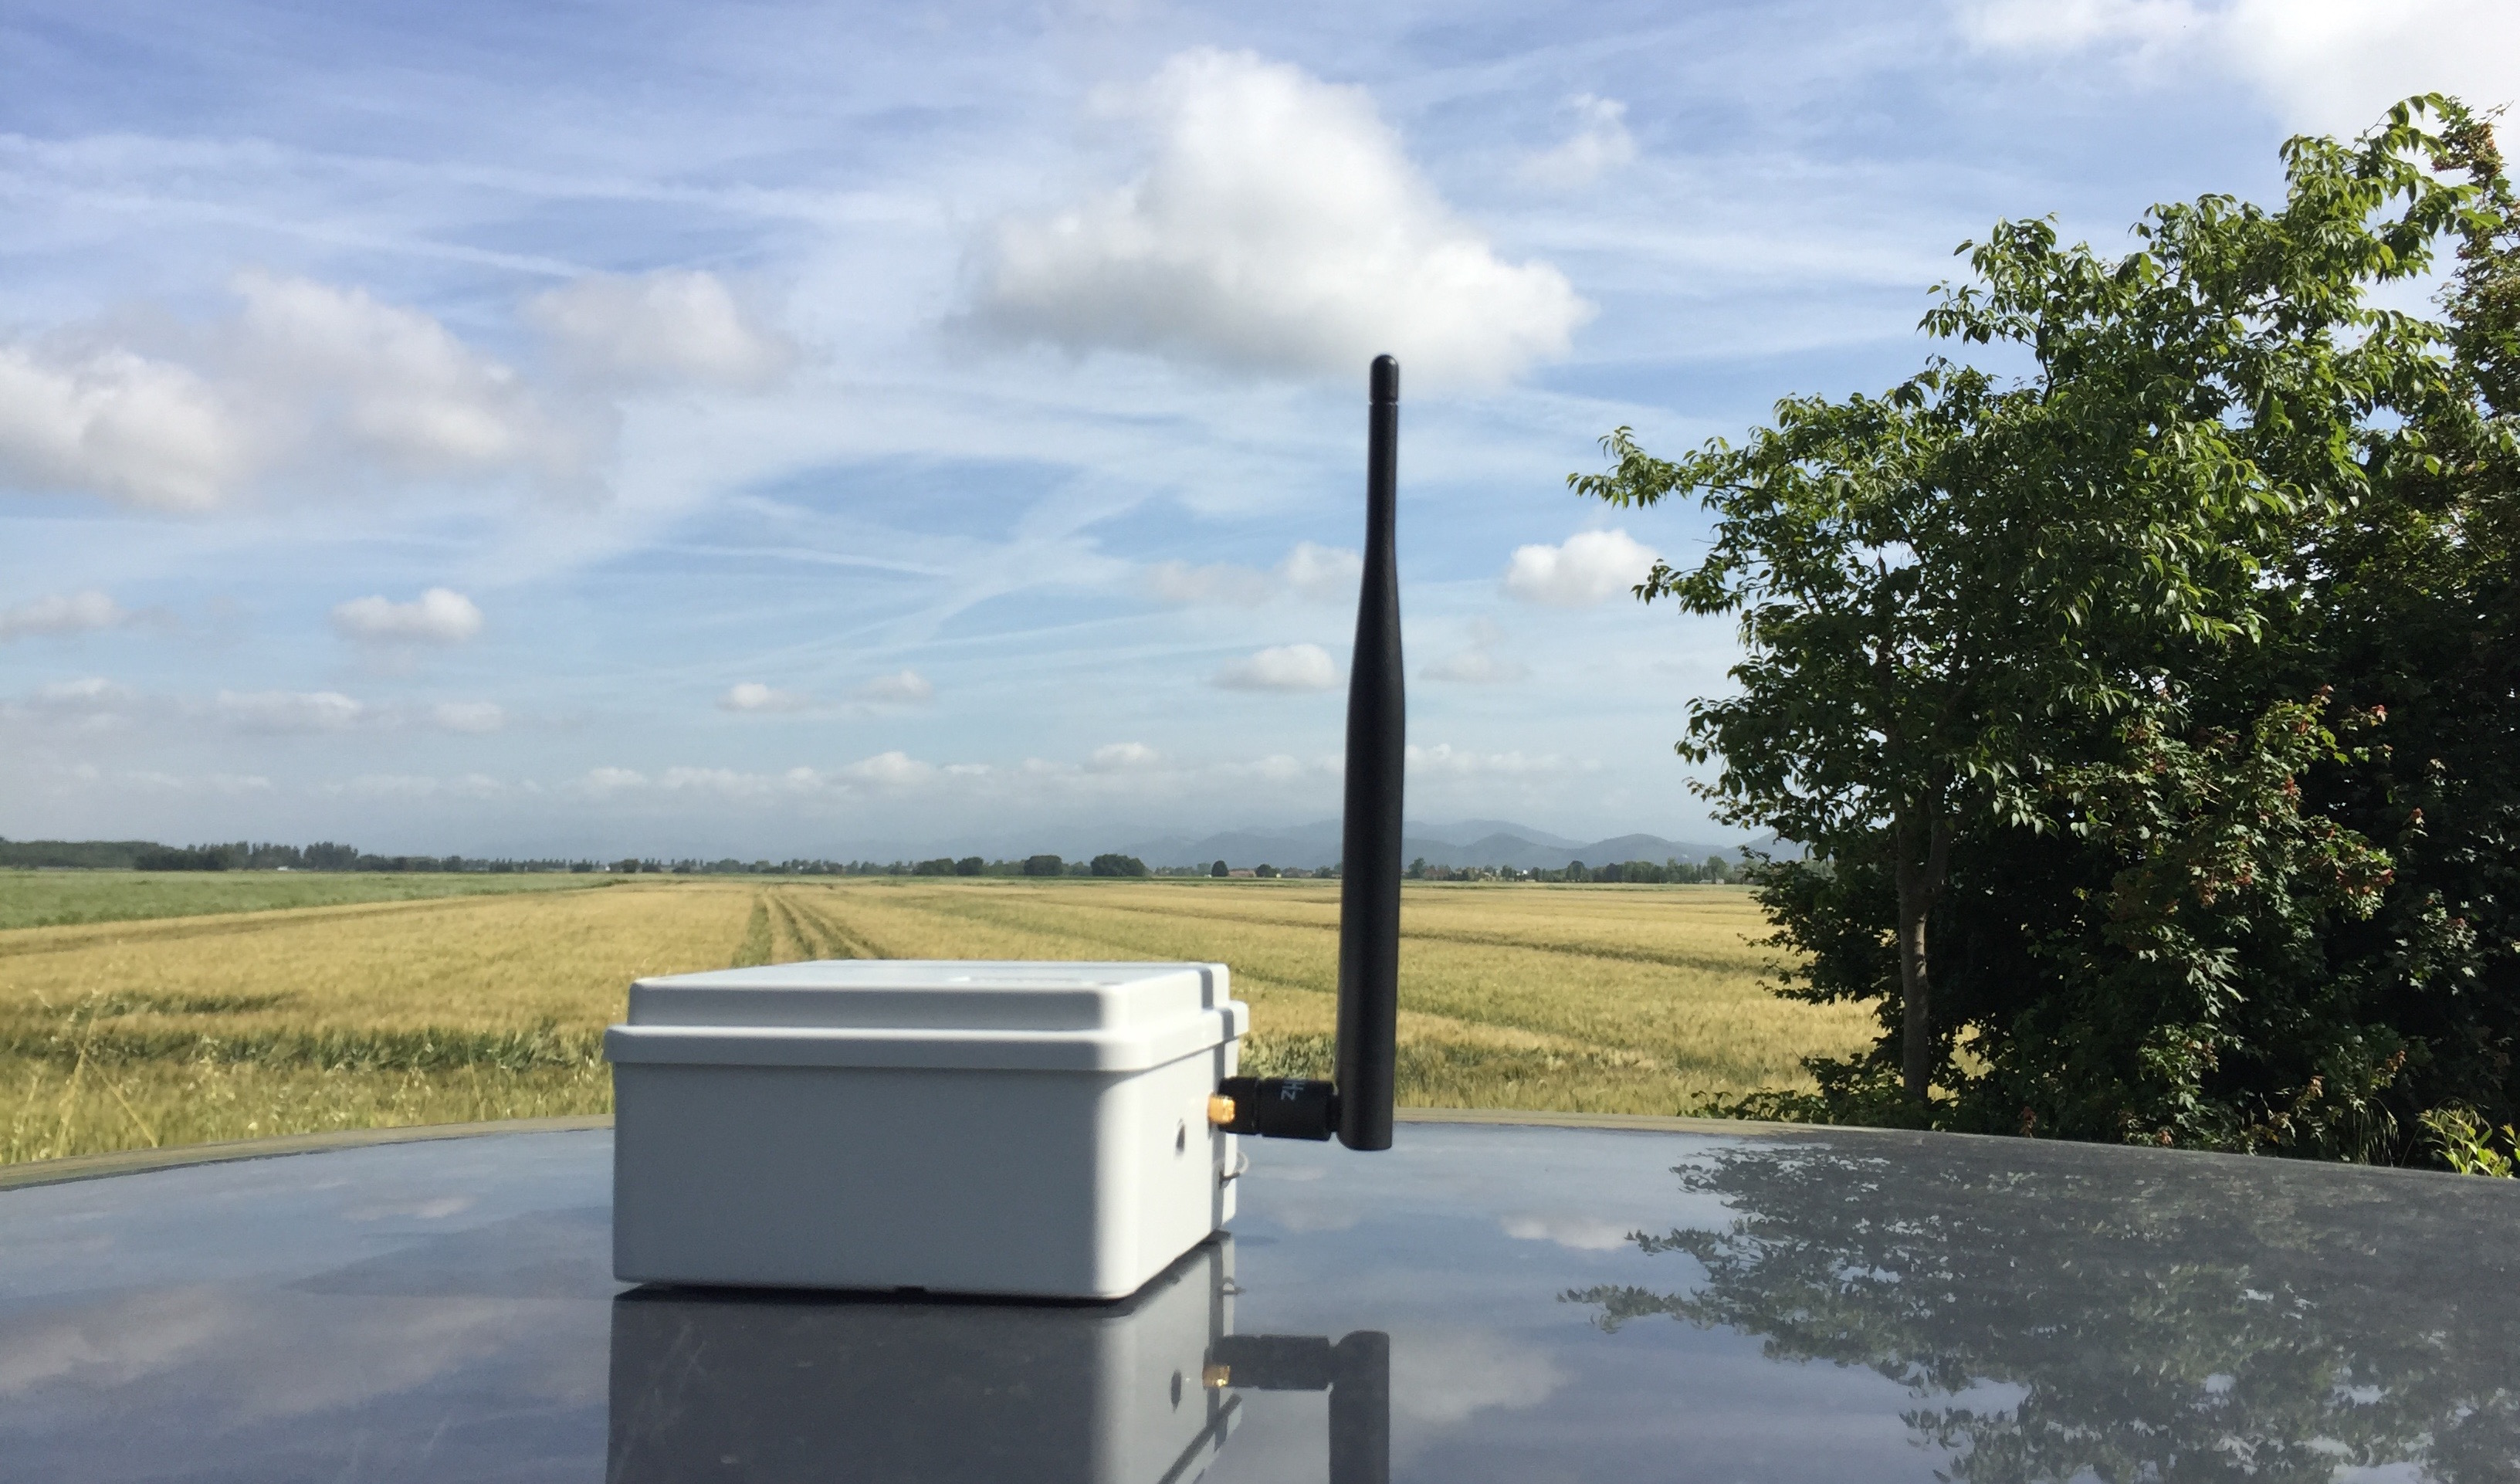
\includegraphics[width=.8\linewidth]{img/mote}
\end{subfigure}
\caption{The Lorank gateway and the Waspmote end-device}
\label{fig:test}
\end{figure}

The first set of experiments was performed in a rural environment with non line of sight condition. The gateway was placed on the terrace of the department of information engineering at the University of Pisa, located in Via Caruso 16, Pisa, Italy.

The end-devices were placed in different spots along a road inside the natural park of San Rossore, Pisa (Italy).

\begin{figure}[]
\centering
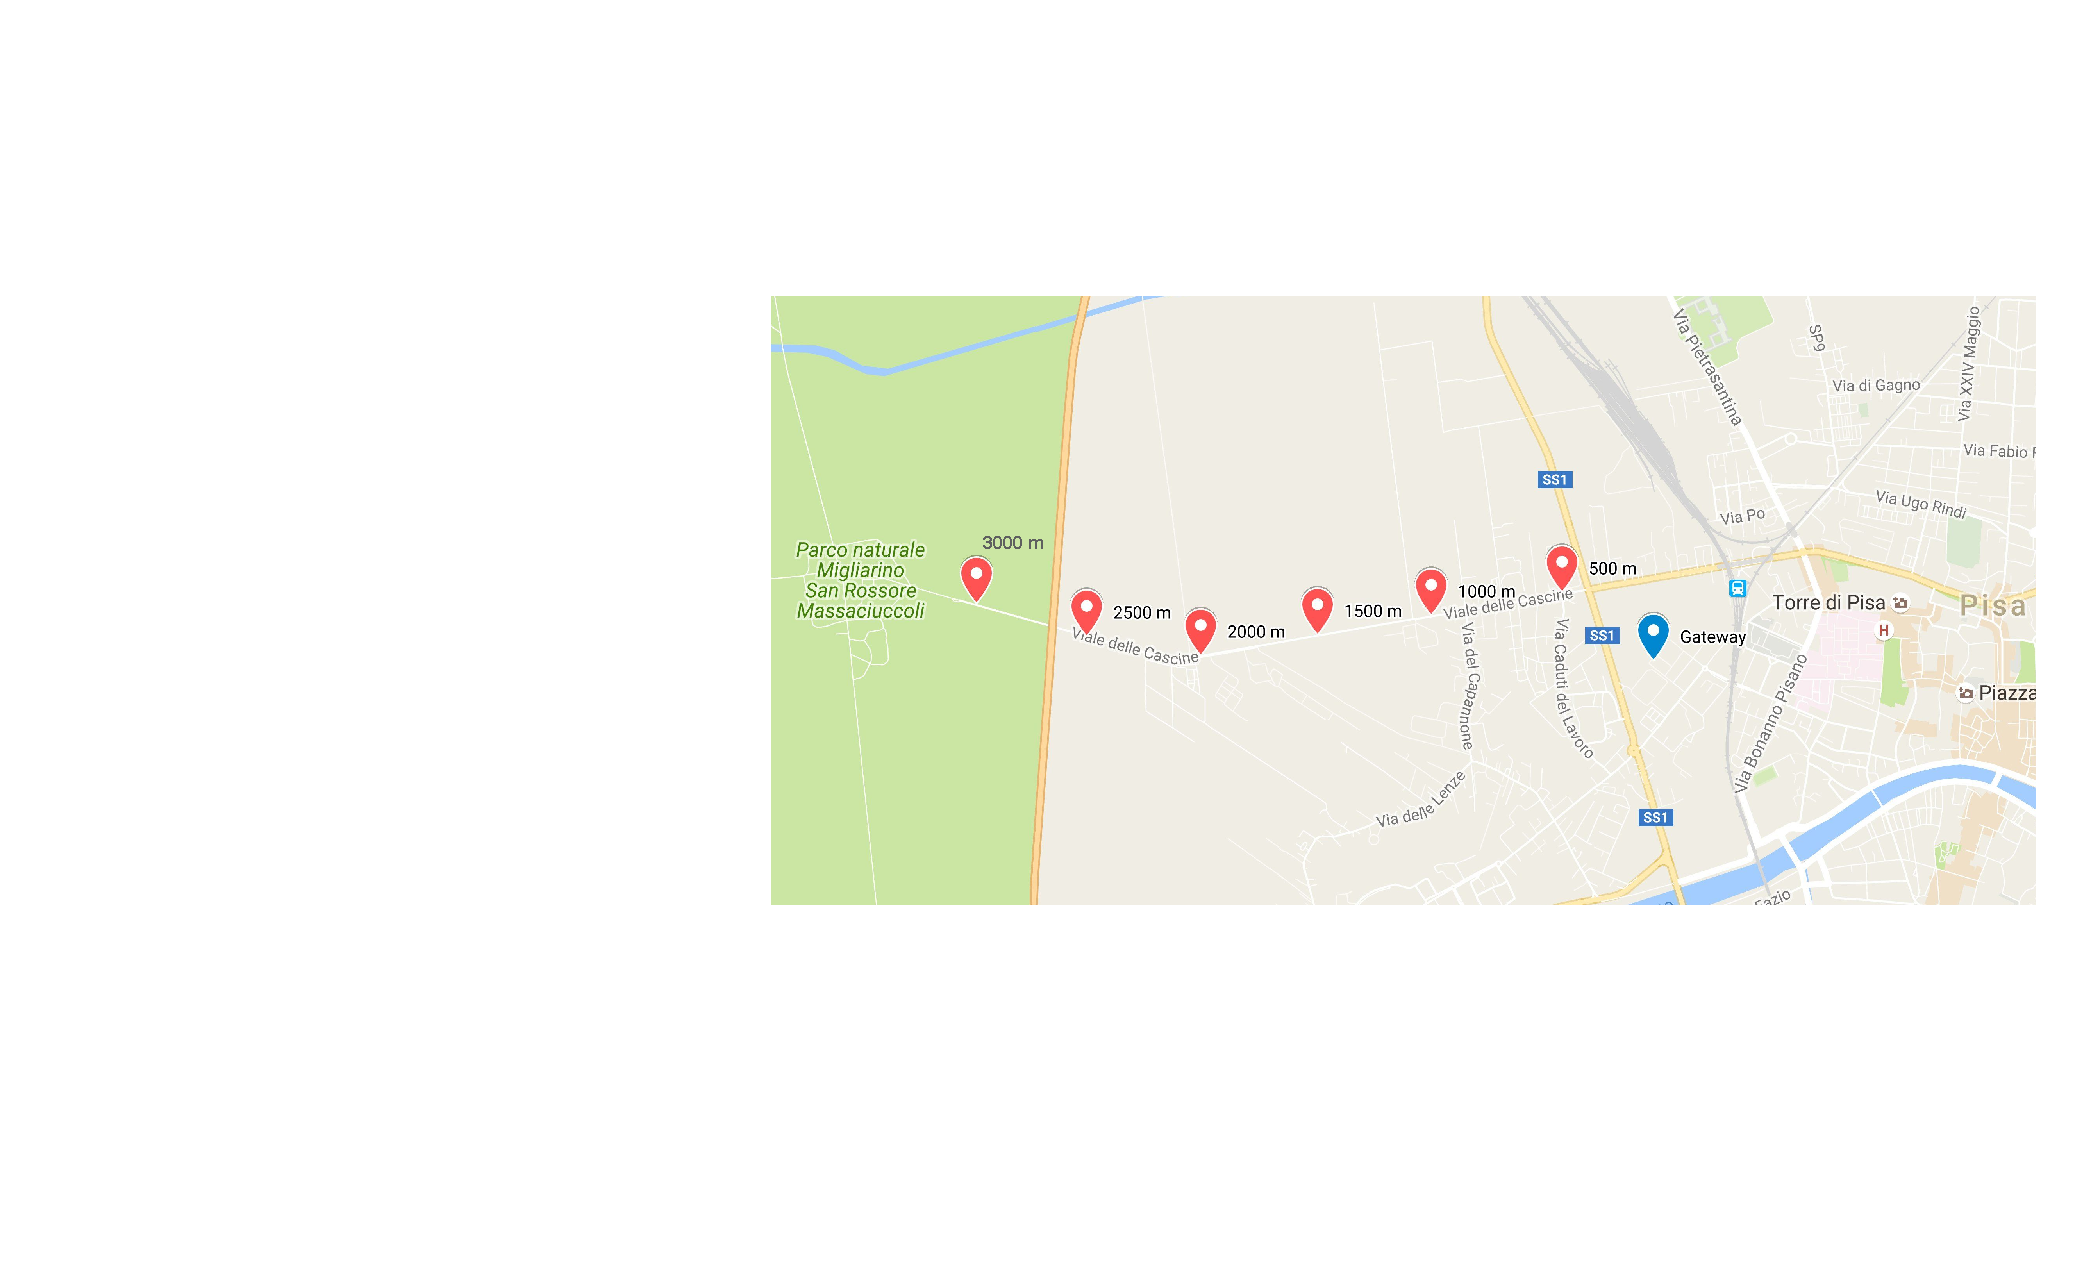
\includegraphics[width=\textwidth]{img/map_rural}
\caption{Map of rural experiments}
\label{fig:maprural}
\end{figure}


\subsection{Selection of parameters} 
Given these particular environments the parameters were chosen as follows:
\begin{itemize}
\item \emph{Data Rate}: all data rates were tested (from SF7BW125 to SF12BW125);
\item \emph{Coding Rate}: since in some preliminary tests it was discovered that the influence of the coding rate on the packet error rate in this environment was negligible, it was decided to test only 4/5;
\item \emph{Distance}: each end-device was placed starting from 500 meters away from the gateway up to 2500 meters, in steps of 500 meters;
\item \emph{Payload length}: 10 bytes and 50 bytes, to cover different real use cases;
\item \emph{Transmission power}: It was decided to test both the highest transmission power available and the lowest for which it is known from preliminary experiments to be strong enough to receive data.

So at 14 dBm and 8 dBm were tested at 1500, 2000 and 2500 meters. At 1000 meters 14 dBm and 5 dBm were tested, and at 500 meters away from the gateway 8 dBM and 2 dBm were tested.
\end{itemize}
Table \ref{tab:ruraltest} summarizes the chosen parameters.


% Please add the following required packages to your document preamble:
% \usepackage{booktabs}
\begin{table}[]
\centering
\caption{Rural test configurations}
\label{tab:ruraltest}
\begin{tabular}{@{}lll@{}}
\toprule
Parameter           & Values & Unit  \\ \midrule
Spreading factor    & 7, 8, 9, 10, 11, 12  &       \\
Coding Rate    & 4/5  &       \\
Transmission power  & 14, 8, 5 (1 Km), 2 (0.5 Km)  & dBm   \\
Payload length      & 10, 50 & bytes \\
Distance from gateway & 0.5, 1.0, 1.5, 2.0, 2.5 & Km    \\ \bottomrule
\end{tabular}
\end{table}

\subsection{Results}
Analyzing the results of this first set of experiments some peculiar behaviors has been discovered, in particular:
\begin{itemize}
\item up to 1500 meters away from the gateway (figure \ref{fig:sf7rural}) it is possible to transmit with the fastest data rate, which is SF7BW125, without having significant losses;

\item the length of the payload affects significantly the packet error rate only at 2500 meters and only with the slowest data rates, i.e. SF11 and SF12 (figures \ref{fig:sf11rural} and \ref{fig:sf12rural}); 

\item At 500 meters, using data rate SF12, it was obtained an higher packet error rate than the faster, and less robust, data rates. In particular the performances of SF12 are significantly worse than SF11, with the same transmission power, and the results with 8 dBm were slightly worse than same data rate with 2 dBm. This strange results are caused by the electric field intensity and the received power over flat terrain.
\end{itemize}


\begin{figure}[]
\centering
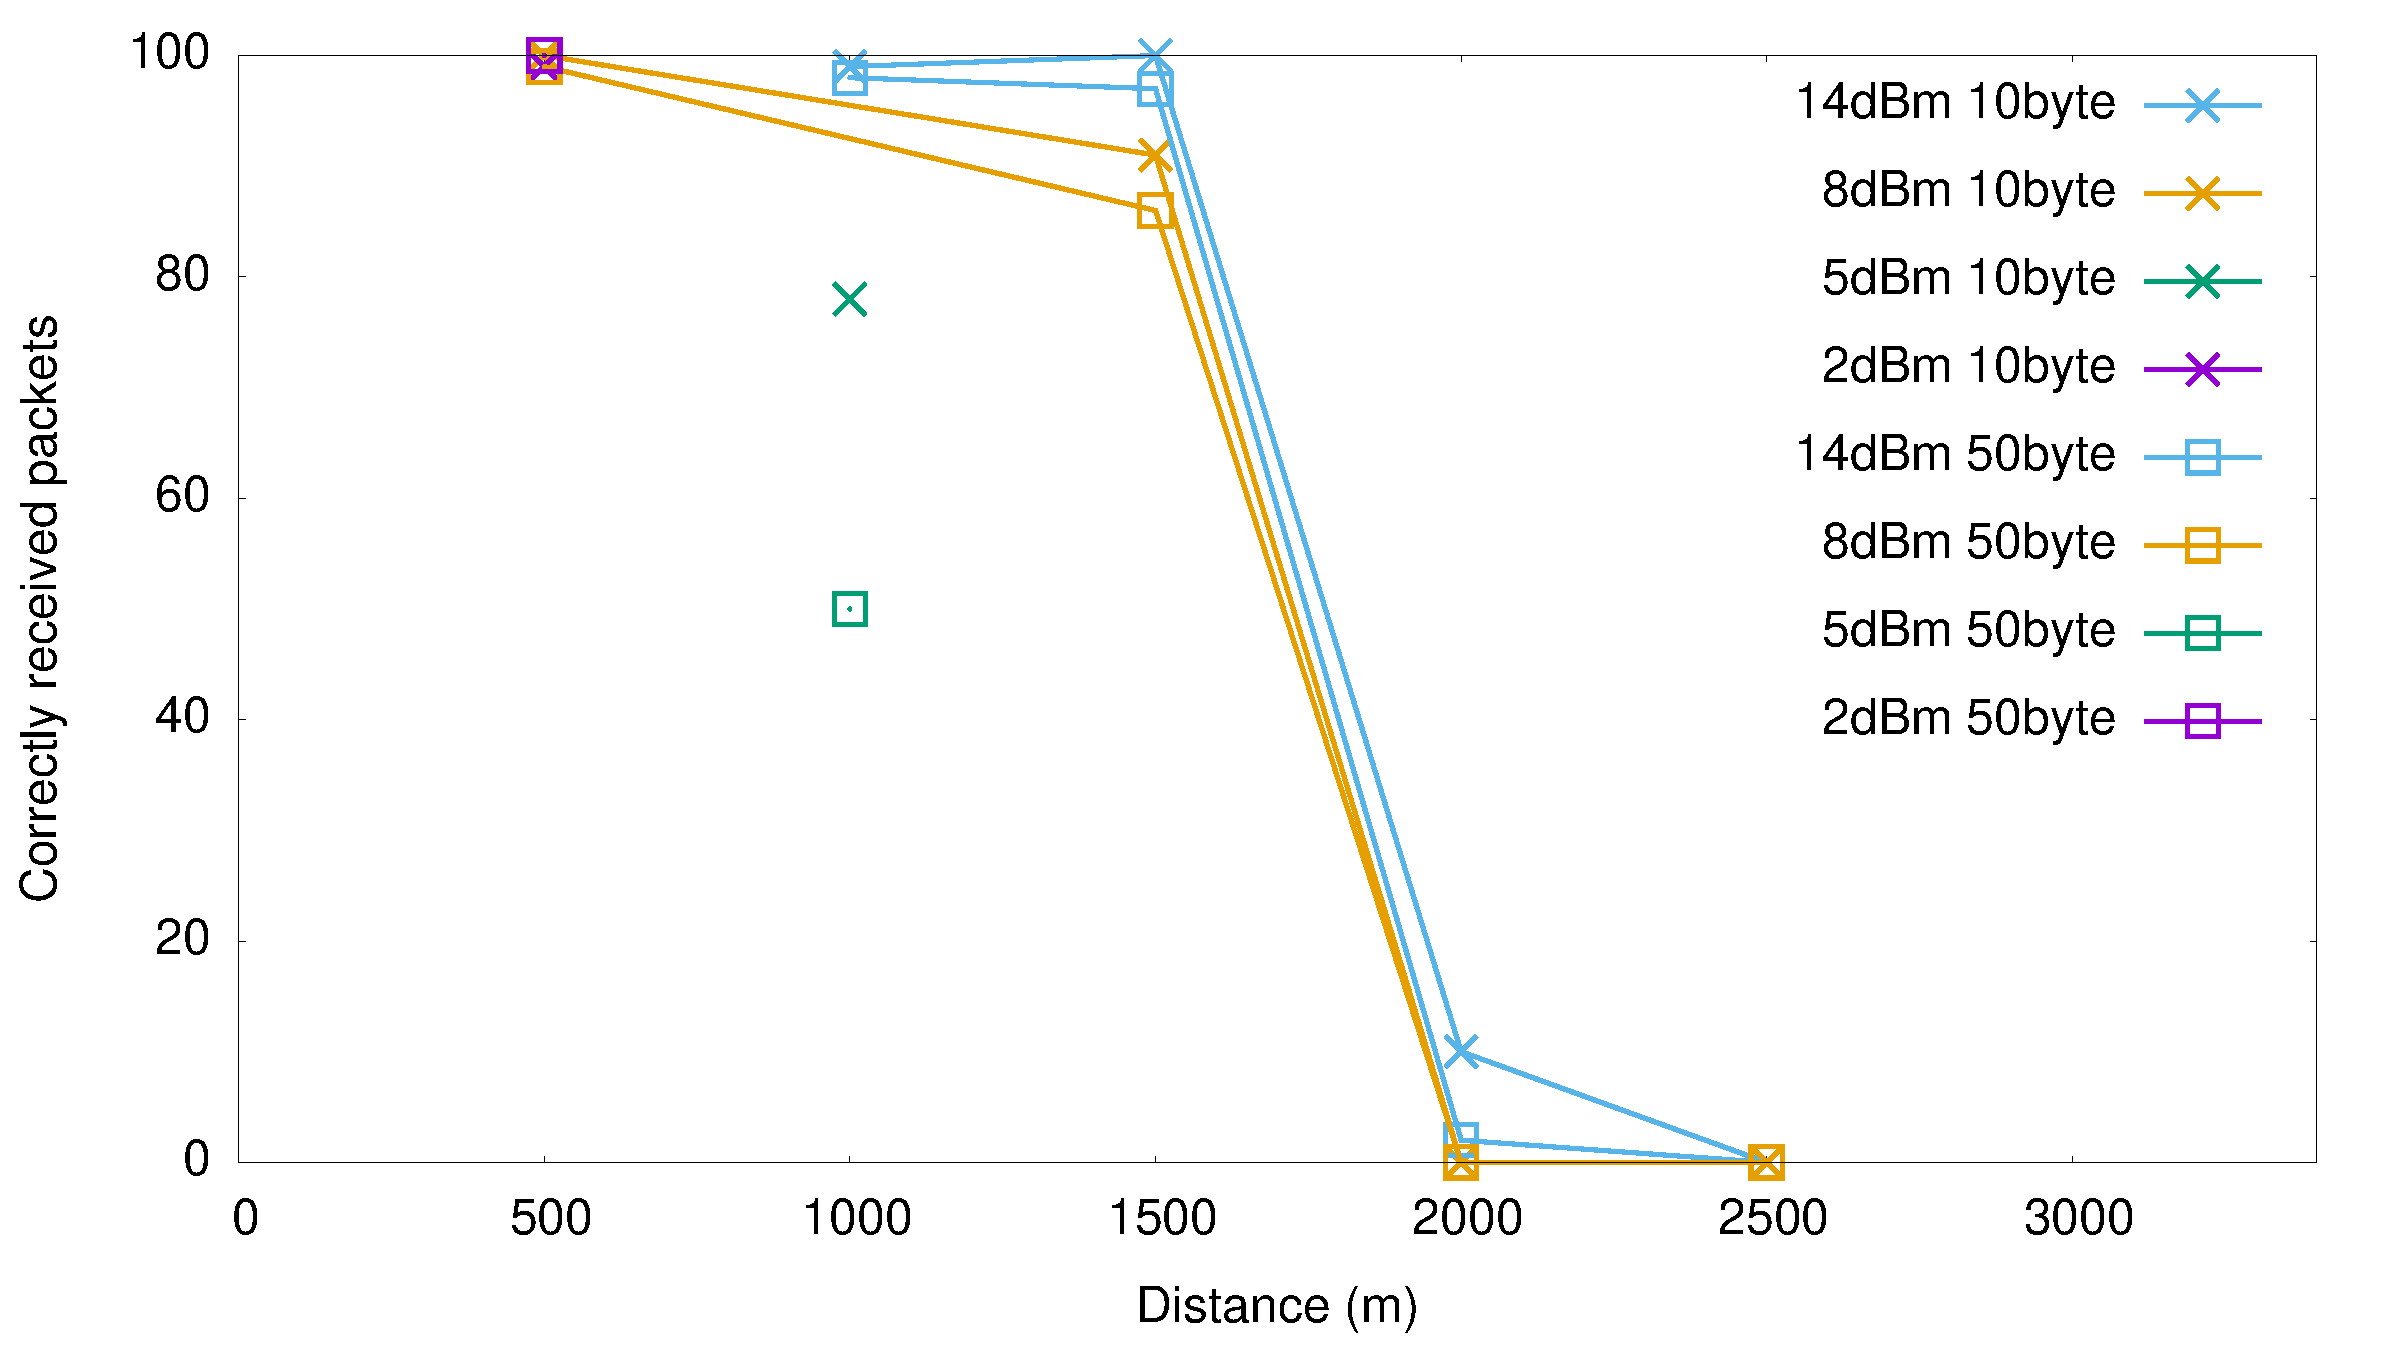
\includegraphics[width=\textwidth]{img/test/rural/sf7}
\caption{Results of rural experiments at SF 7}
\label{fig:sf7rural}
\end{figure}

\begin{figure}[]
\centering
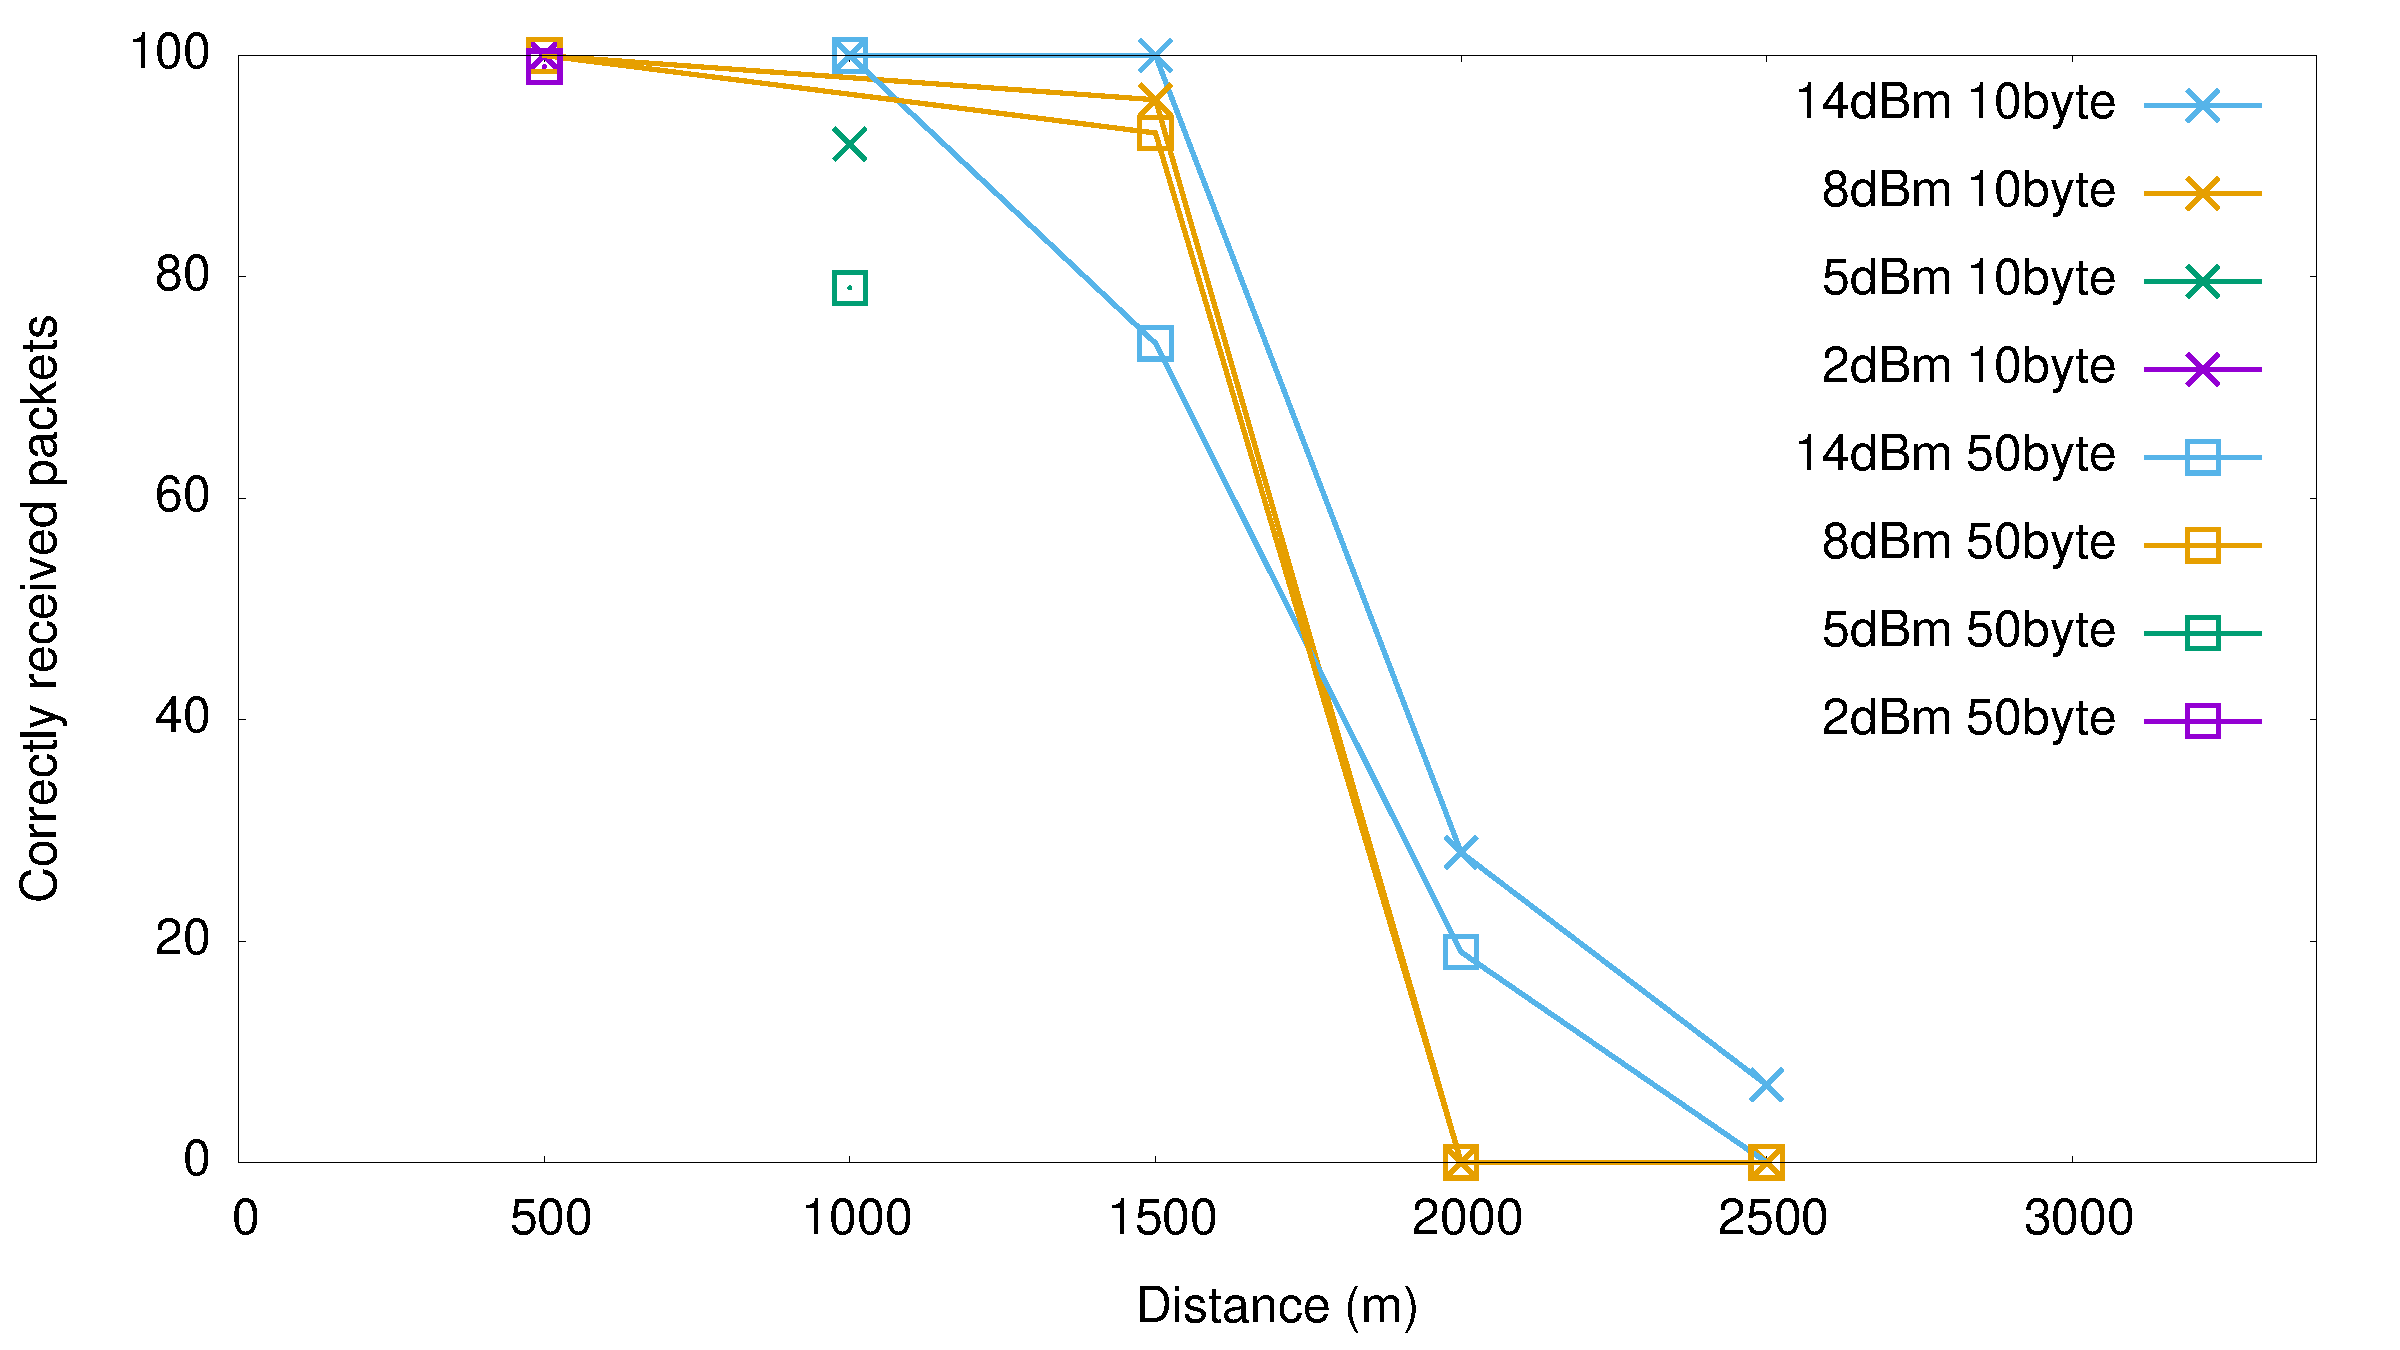
\includegraphics[width=\textwidth]{img/test/rural/sf8}
\caption{Results of rural experiments at SF 8}
\label{fig:sf8rural}
\end{figure}

\begin{figure}[]
\centering
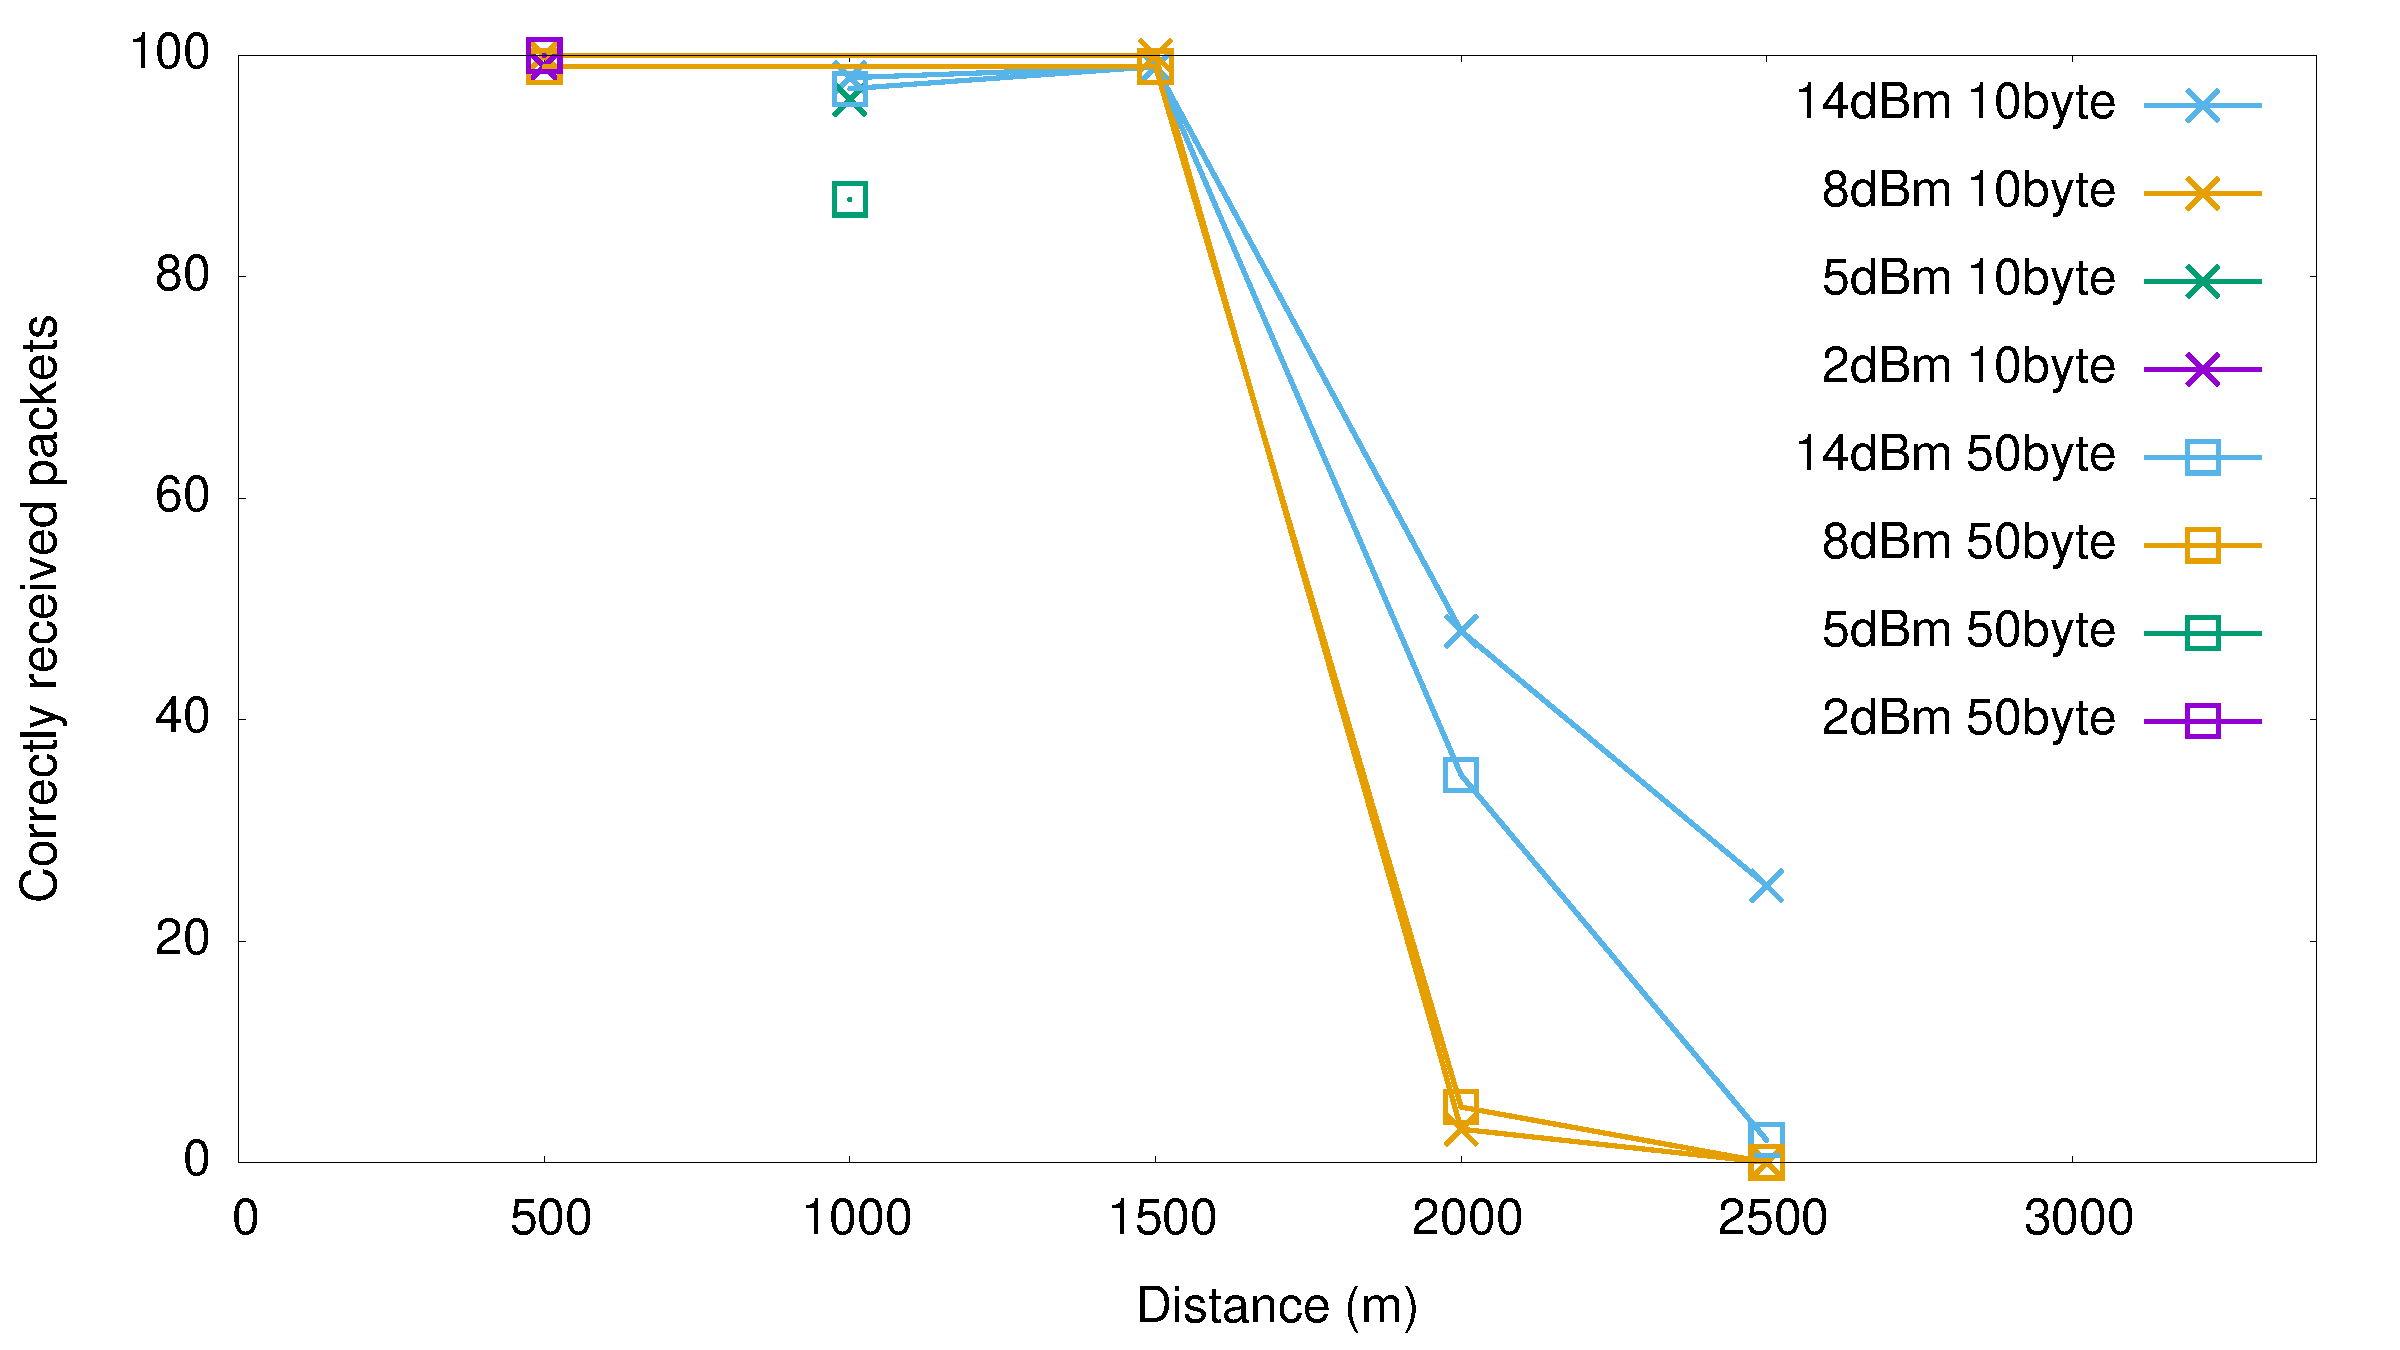
\includegraphics[width=\textwidth]{img/test/rural/sf9}
\caption{Results of rural experiments at SF 9}
\label{fig:sf9rural}
\end{figure}

\begin{figure}[]
\centering
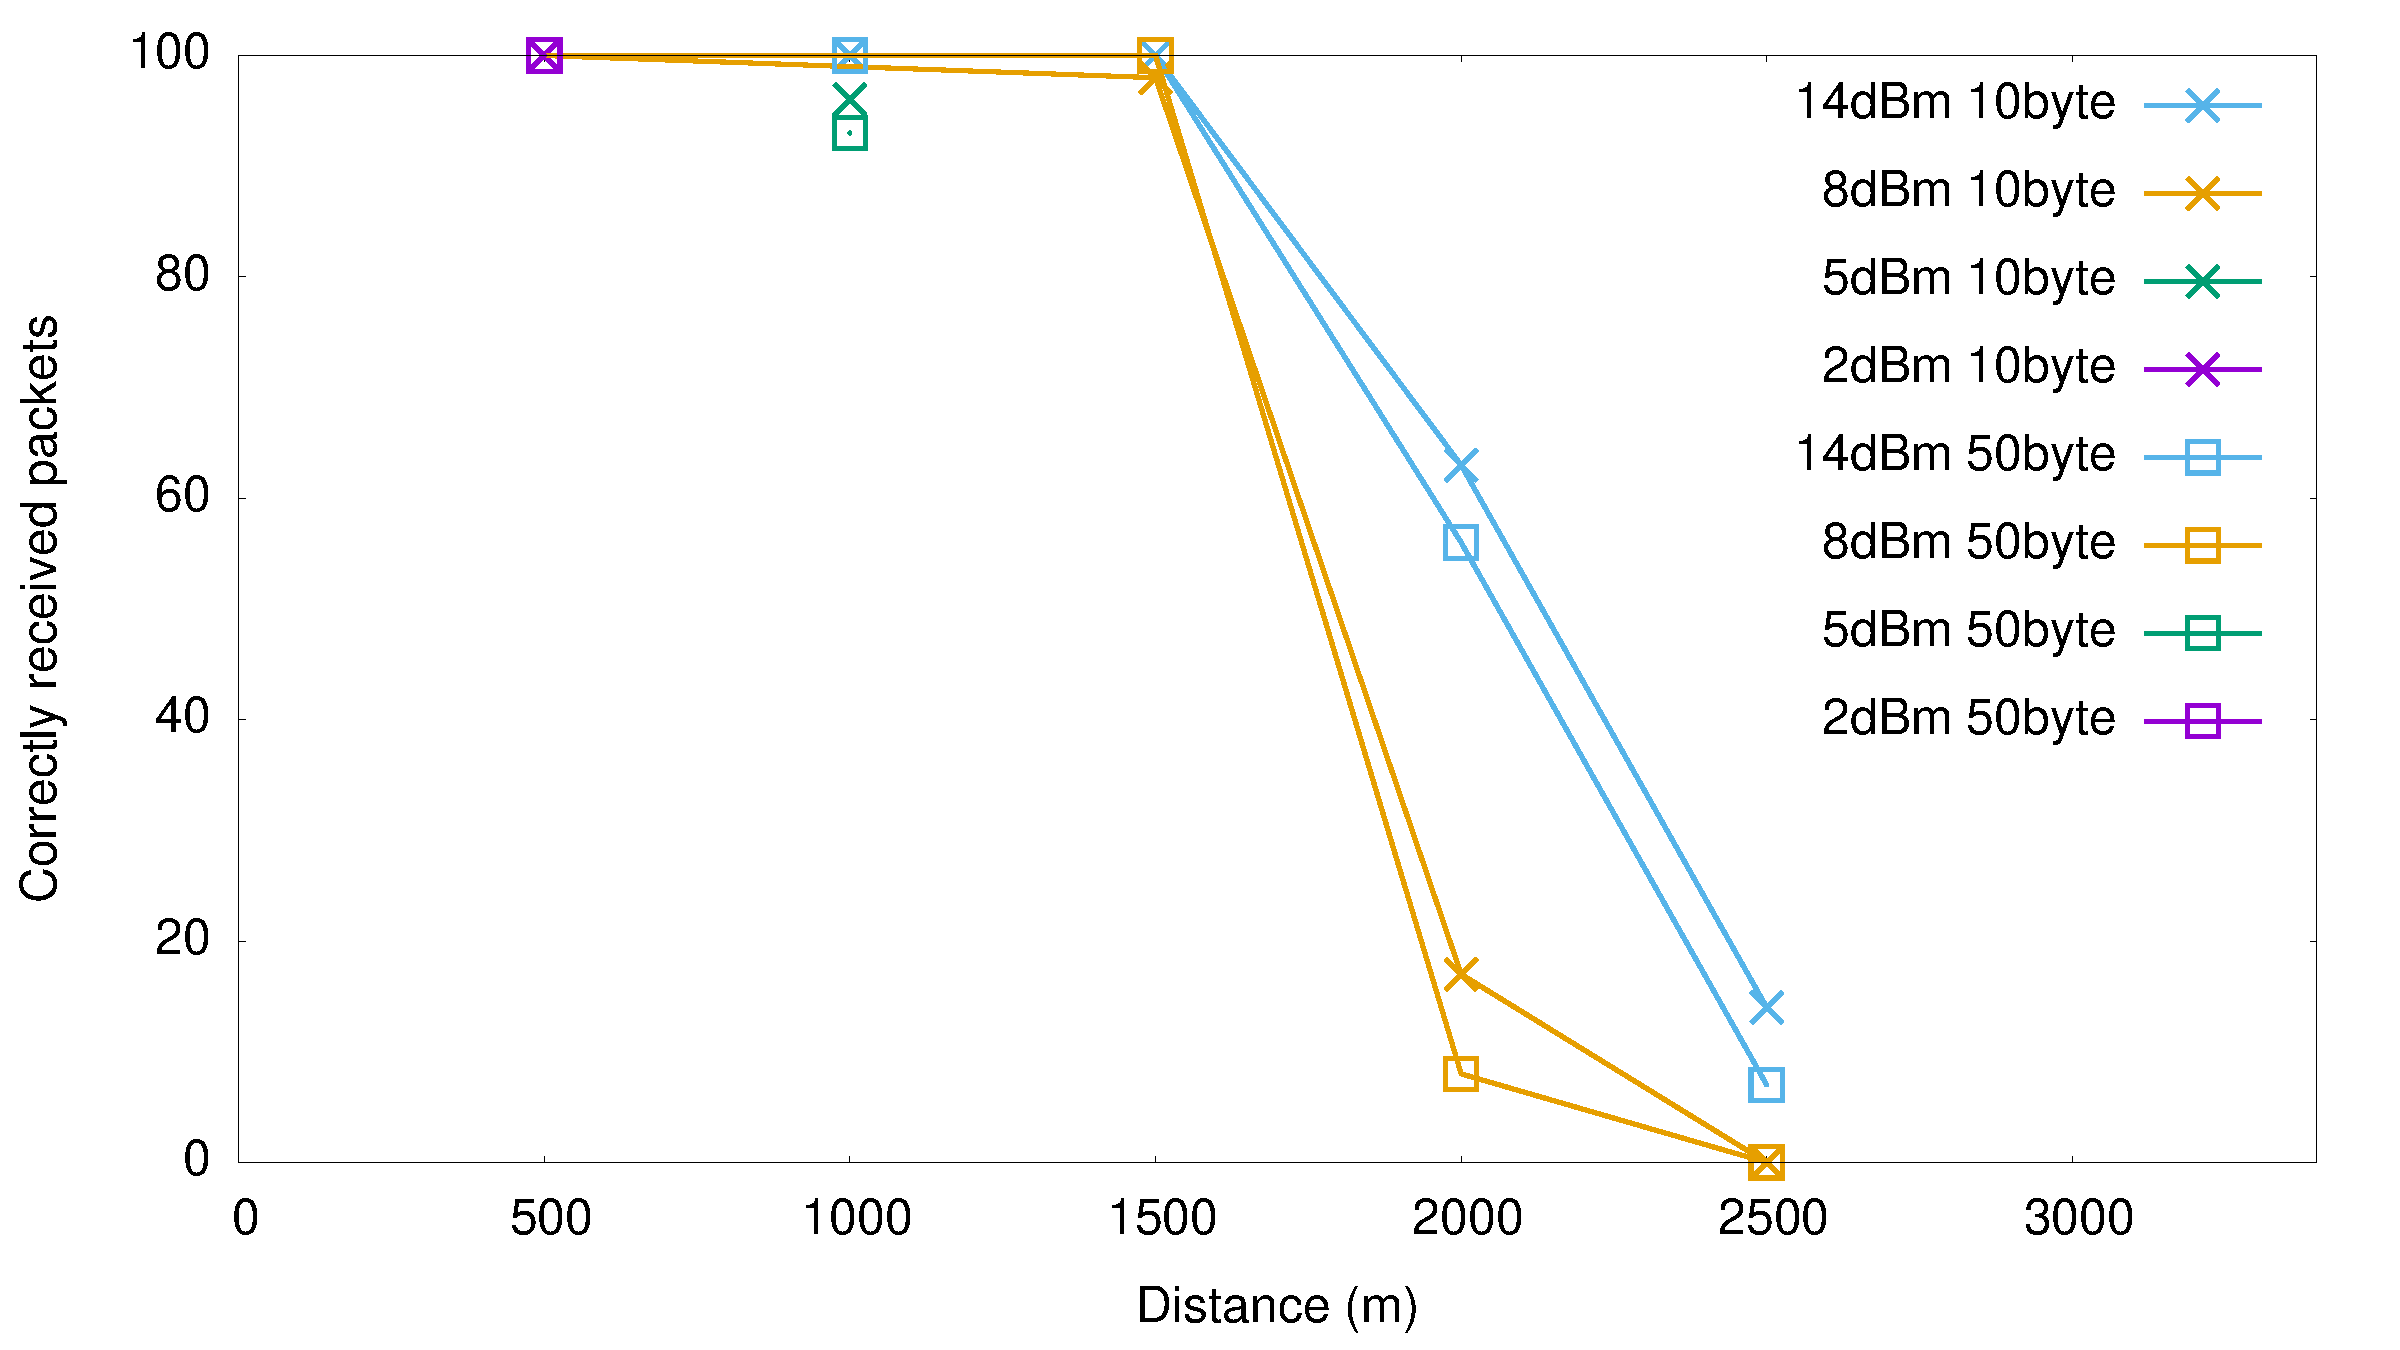
\includegraphics[width=\textwidth]{img/test/rural/sf10}
\caption{Results of rural experiments at SF 10}
\label{fig:sf10rural}
\end{figure}

\begin{figure}[]
\centering
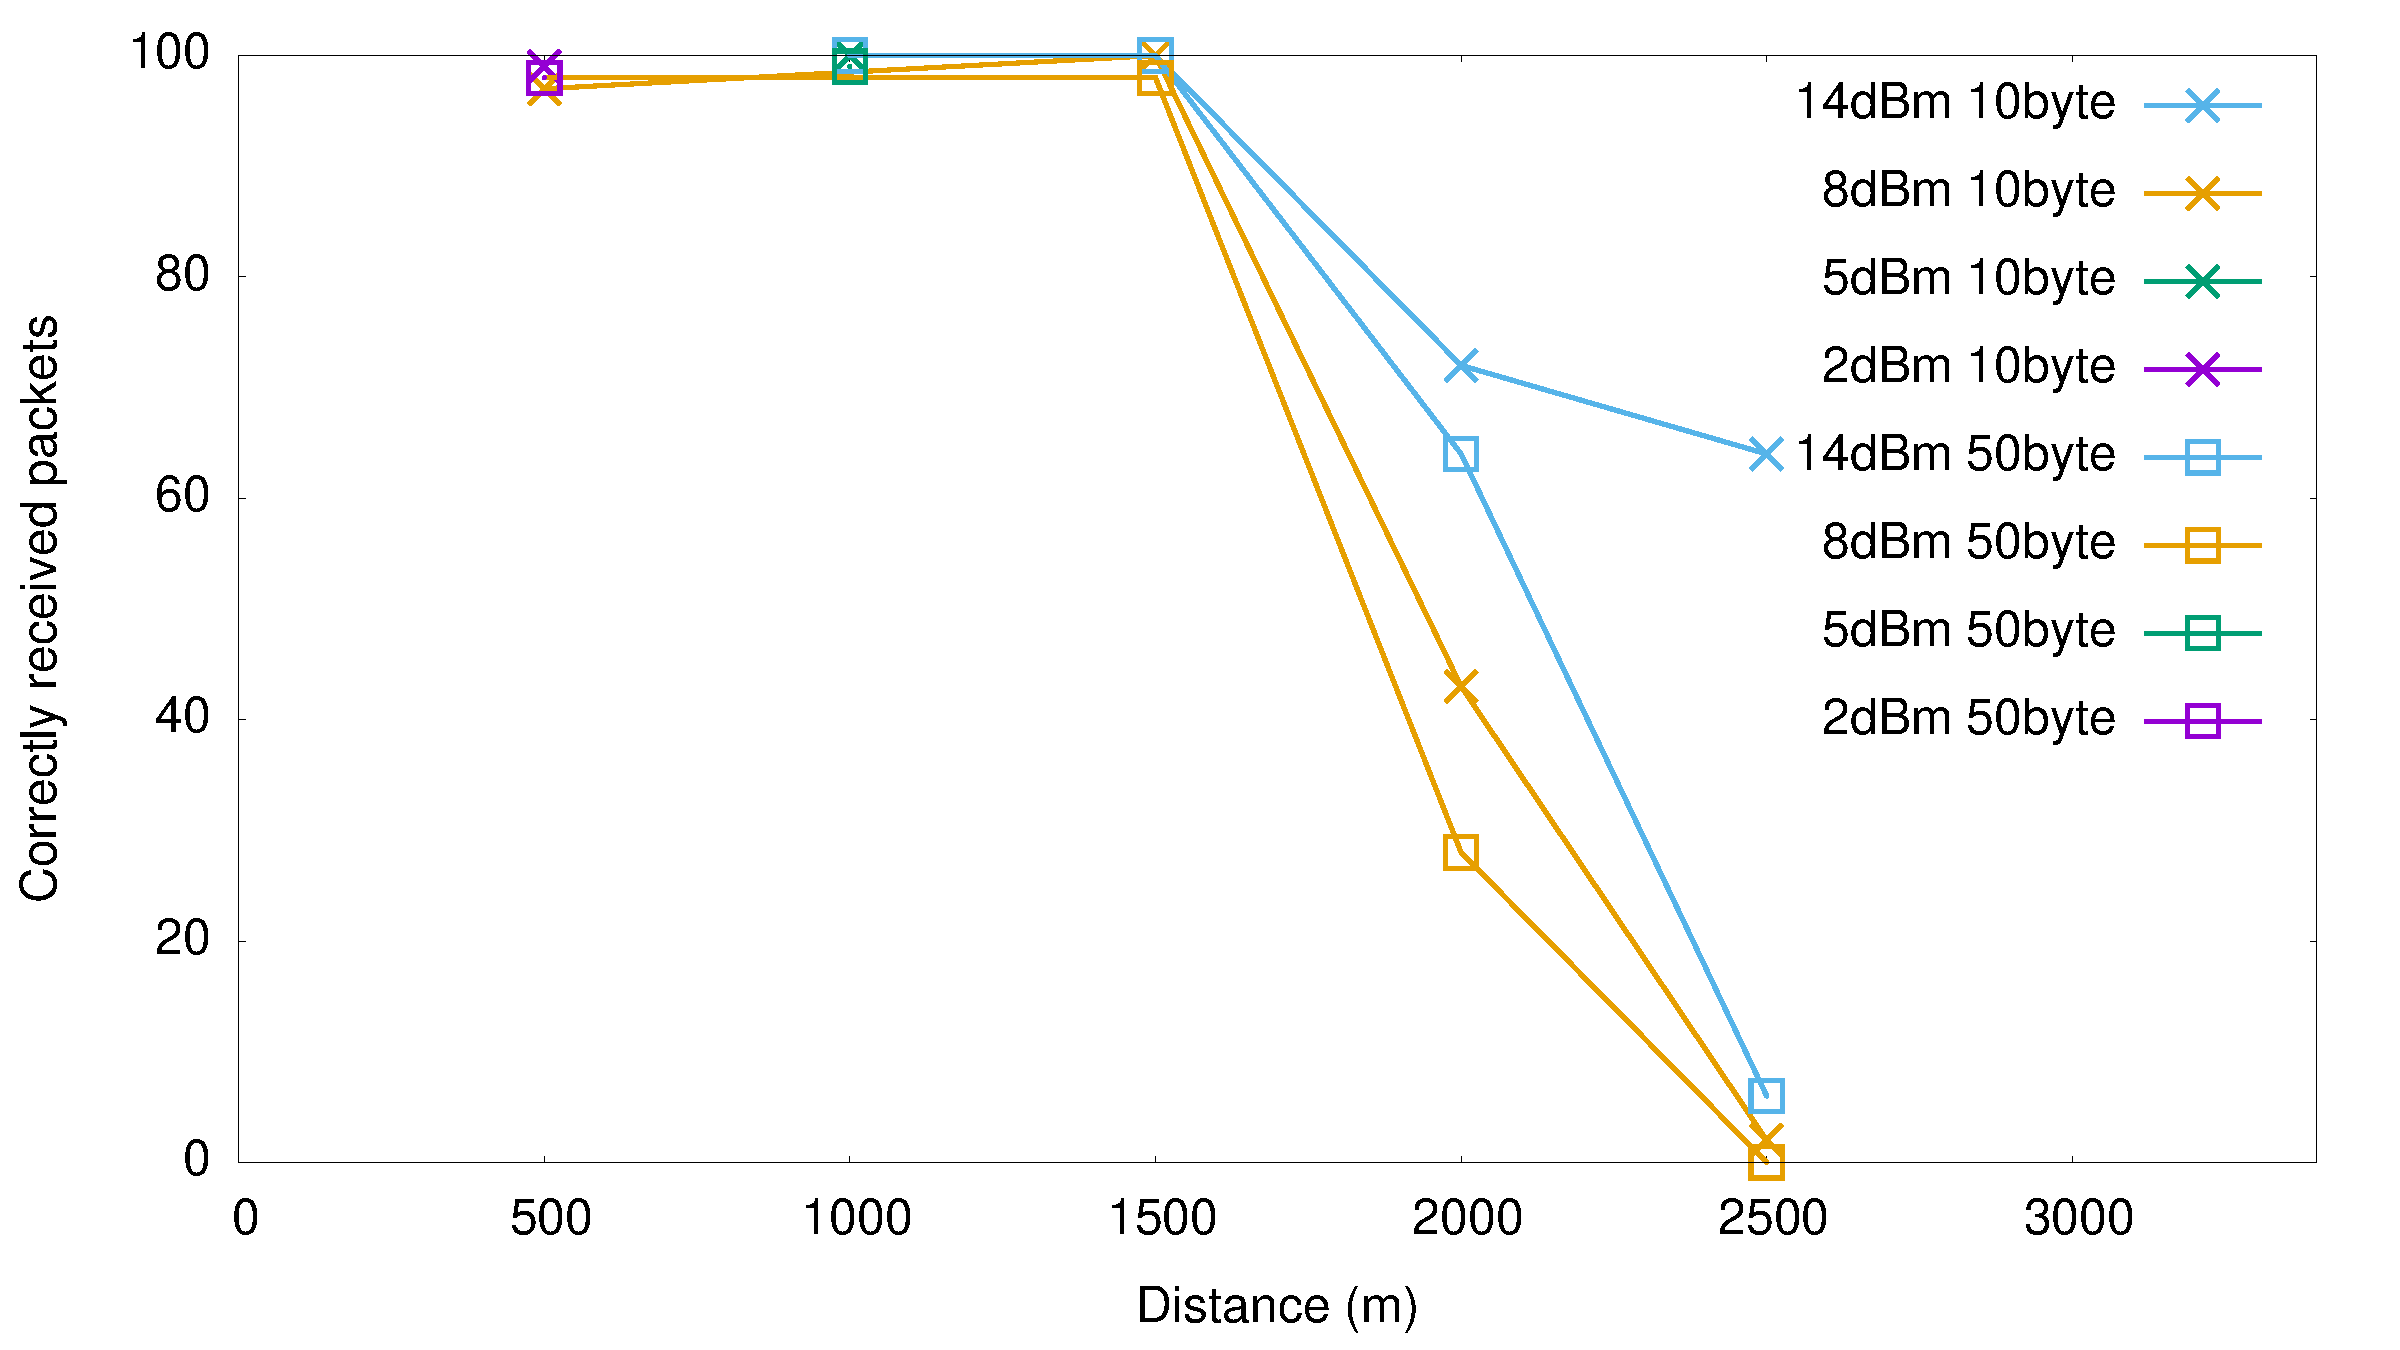
\includegraphics[width=\textwidth]{img/test/rural/sf11}
\caption{Results of rural experiments at SF 11}
\label{fig:sf11rural}
\end{figure}

\begin{figure}[]
\centering
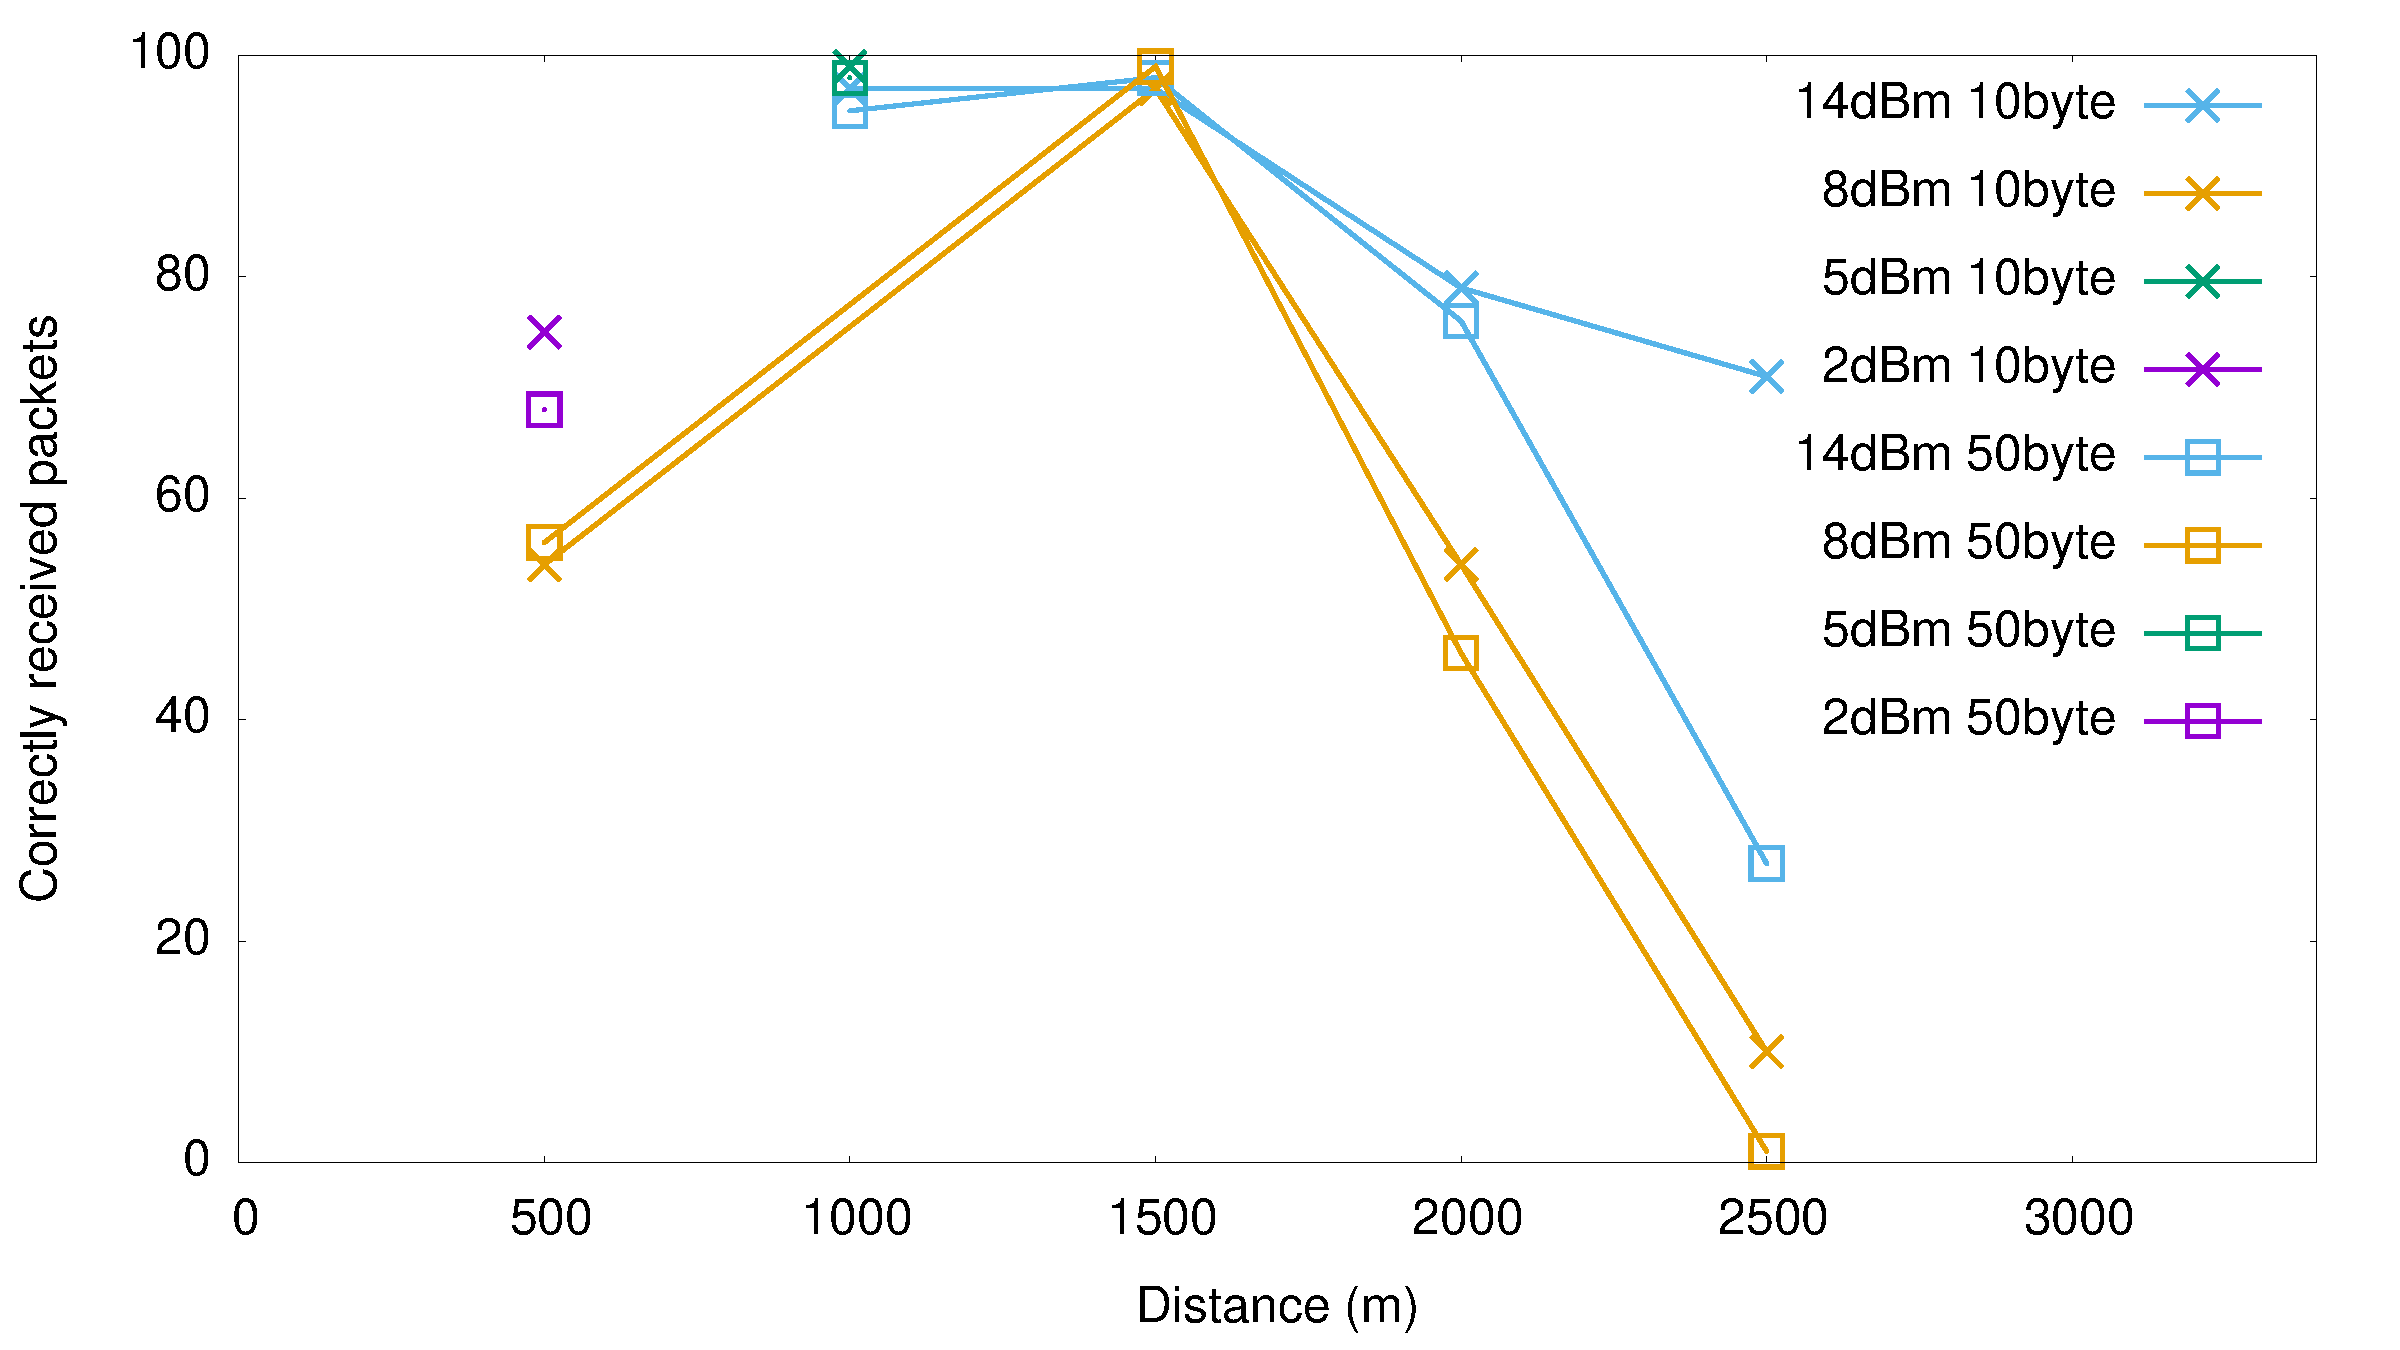
\includegraphics[width=\textwidth]{img/test/rural/sf12}
\caption{Results of rural experiments at SF 12}
\label{fig:sf12rural}
\end{figure}


\newpage
\section{Urban experiments}

The urban experiments were performed in the city center of Pisa. The gateway was placed in front of a window at the fifth floor of department of information engineering, section computer engineering, at the University of Pisa, located in Largo Lucio Lazzarino 1, Pisa, Italy.

The end-device was placed inside, at the first floor of a building located in Via Risorgimento, Pisa. The area between the two devices is a typical urban area with three-floor buildings in the middle.

\begin{figure}[]
\centering
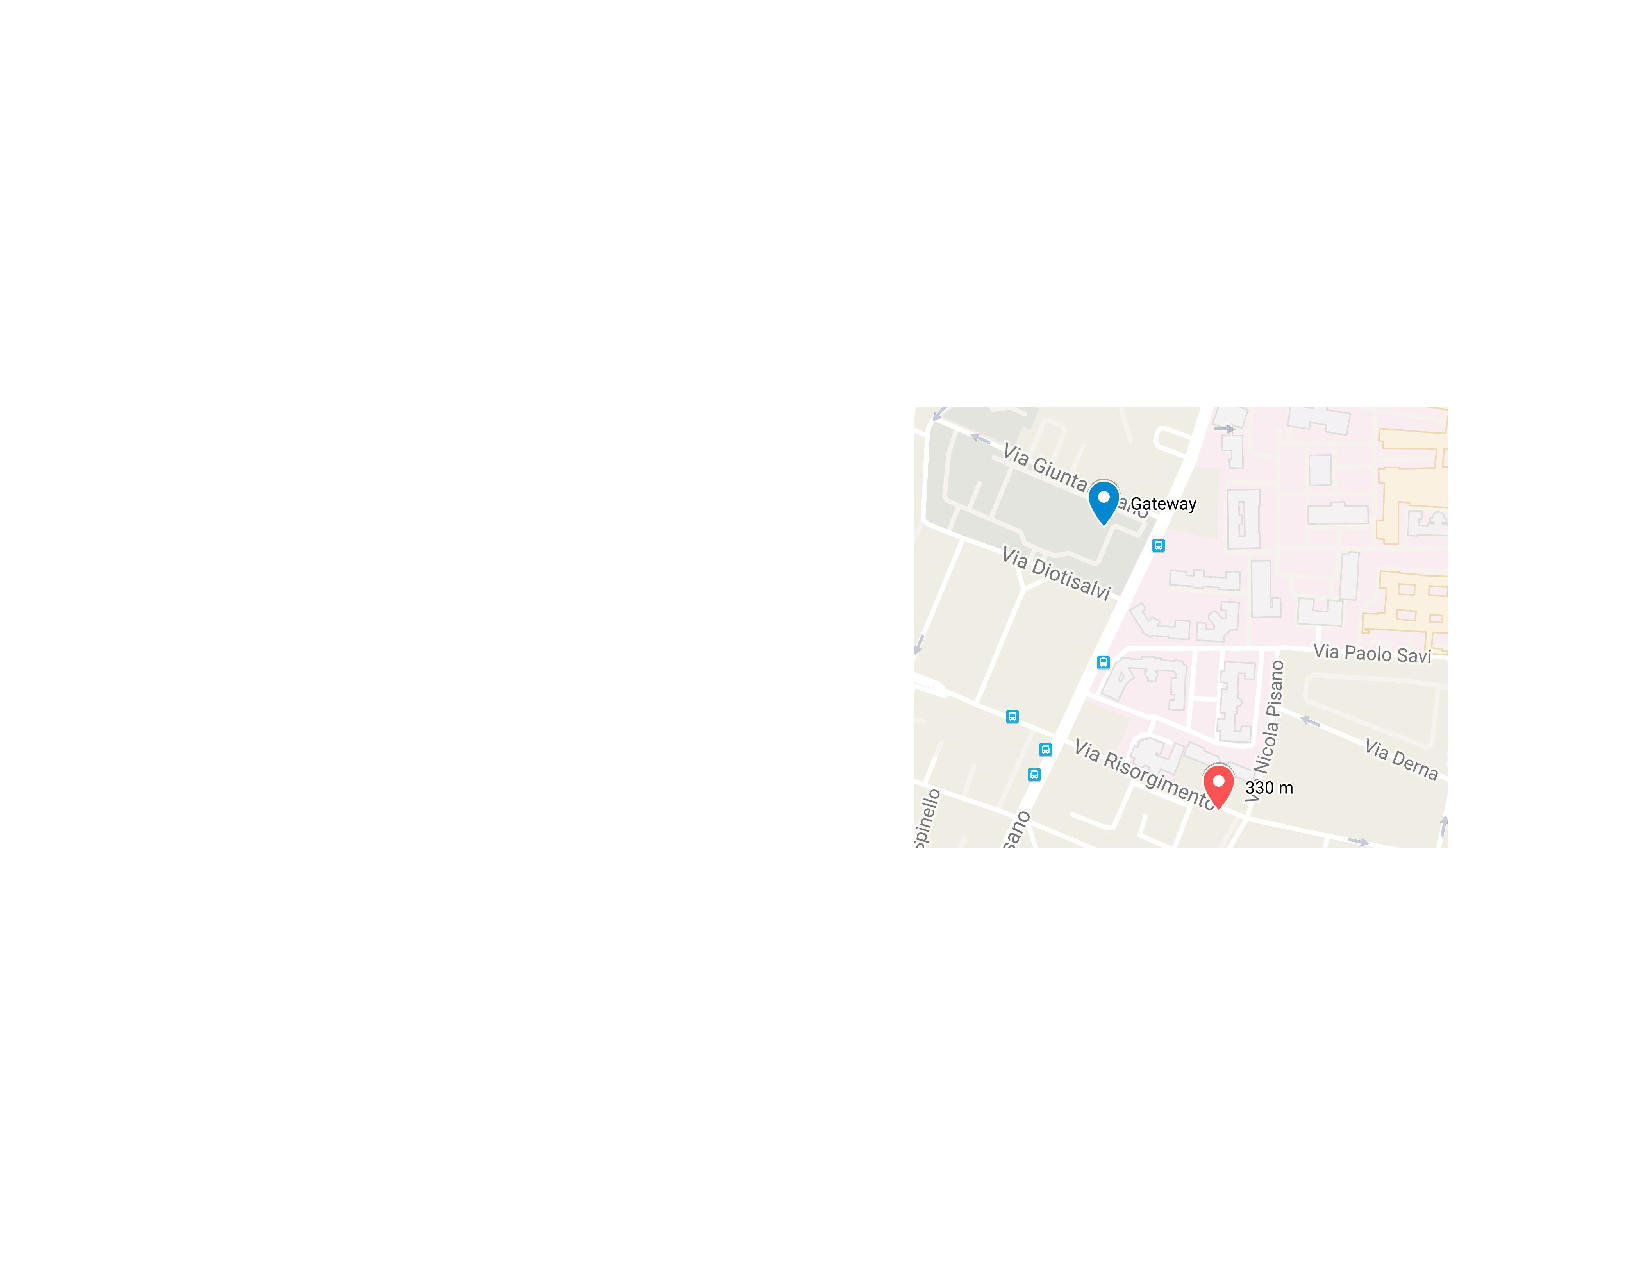
\includegraphics[width=.7\textwidth]{img/map_urban}
\caption{Map of urban experiments}
\label{fig:mapurban}
\end{figure}


\subsection{Selection of parameters} 

For this set of experiments, rather than distances with fixed steps, it was decided to choose some fixed location and try to test all possibles configurations. Since the range of coverage is substantially smaller than in rural test, it was decided also to evaluate the impact of an higher forward error correction, determined by the coding rate, on the reliability of the link.

The parameters were chosen as follows:
\begin{itemize}
\item \emph{Data Rate}: all data rates were tested (from SF7BW125 to SF12BW125);
\item \emph{Coding Rate}: the lowest level of FEC, 4/5, and the highest one, 4/8, were tested;
\item \emph{Distance}: each end-device was placed in a fixed location inside a building; in this section are presented only the results obtained at 330 meters away from the gateway;
\item \emph{Payload length}: 10 bytes and 50 bytes, to cover different real use cases;
\item \emph{Transmission power}: 14, 8, 5, 2 dBm in order to complete explore the impact of the reduction of transmission power on the packet error rate.
\end{itemize} 
Table \ref{tab:urbantest} summarizes the chosen parameters.

% Please add the following required packages to your document preamble:
% \usepackage{booktabs}
\begin{table}[]
\centering
\caption{Urban test configurations}
\label{tab:urbantest}
\begin{tabular}{@{}lll@{}}
\toprule
Parameter           & Values & Unit  \\ \midrule
Spreading factor    & 7, 8, 9, 10, 11, 12  &       \\
Coding Rate    & 4/5, 4/8  &       \\
Transmission power  & 14, 8, 5, 2  & dBm   \\
Payload length      & 10, 50 & bytes \\
Distance from gateway & 0.33 & Km    \\ \bottomrule
\end{tabular}
\end{table}


\subsection{Results}
From the results of this experiments it is possible to notice that, as expected, transmission with an higher level of \emph{forward error correction} are more reliable than the other ones, but in general the variation of the \emph{coding rate} does not substantially improve performance, especially with shorter packets;

However, in border cell condition the impact of the \emph{coding rate} is considerably high. It is possible to appreciate this behavior in particularly for spreading factor 9 (figure \ref{fig:sf9urban}): considering experiments with payload of 50 bytes, it is possible to notice that in extreme conditions, i.e. the best and worst transmission power, there is no difference of behavior between two different coding rates. Instead, for 5 and 8 dBm, the higher coding rate makes really the difference, making the channel a lot more reliable than with lower coding rate.

Regarding the other parameters, both \emph{payload length} and \emph{transmission power} behaved as expected from theory.

\begin{figure}[]
\centering
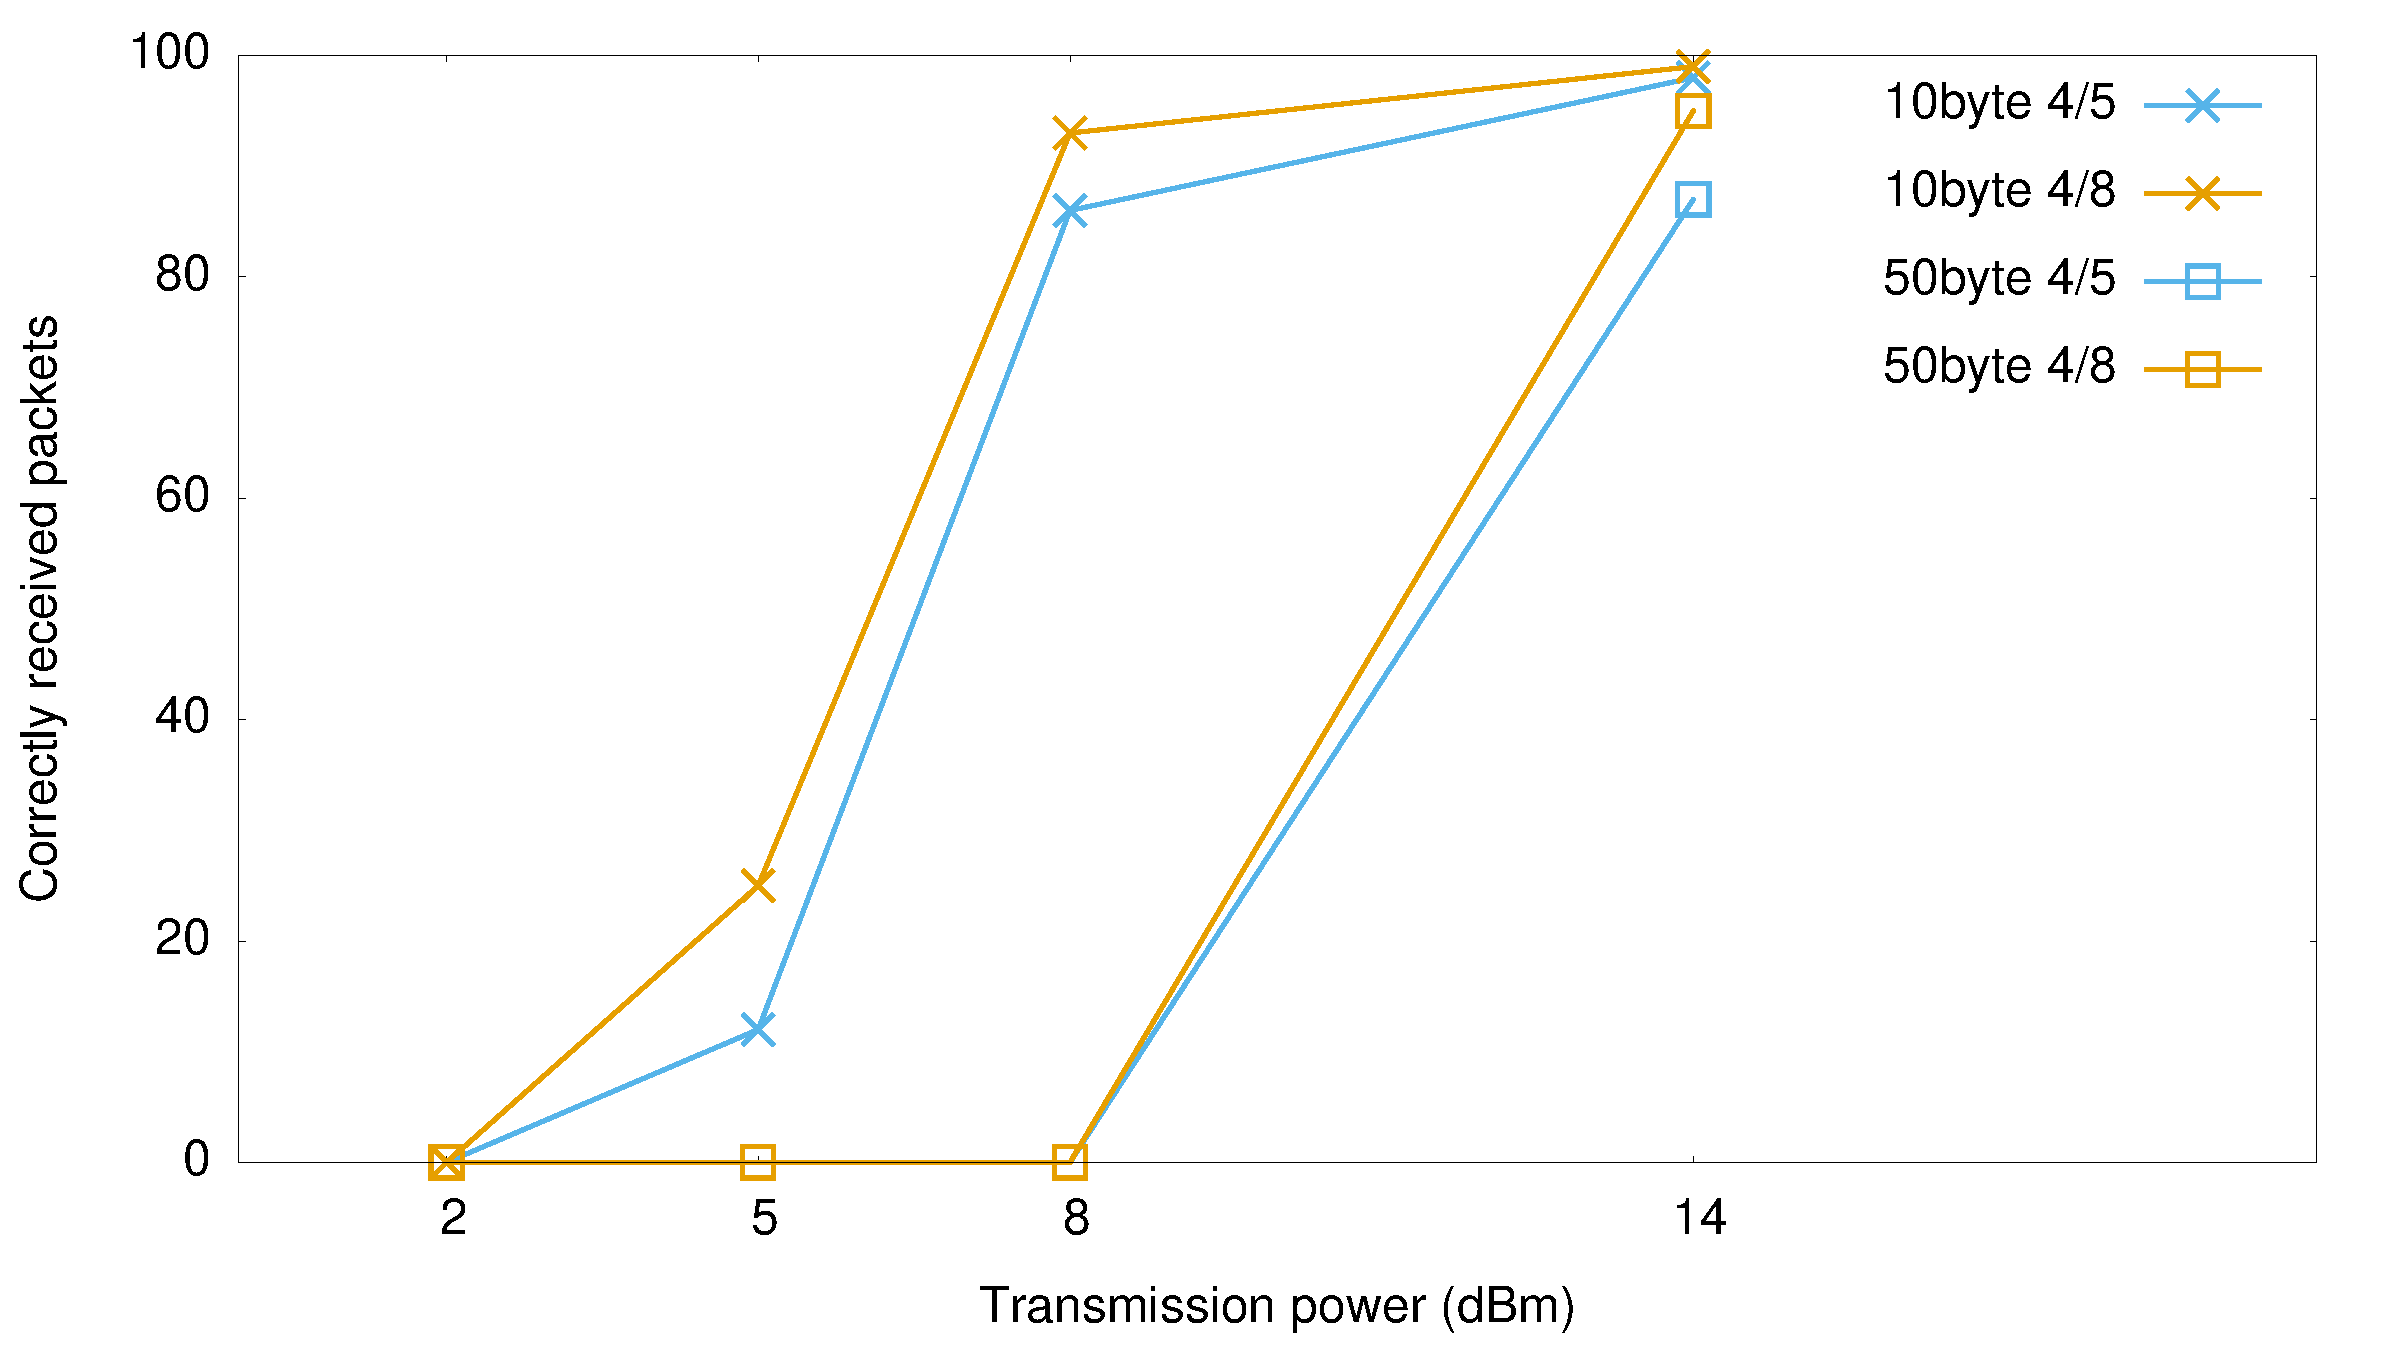
\includegraphics[width=\textwidth]{img/test/urban/sf7}
\caption{Results of urban experiments at SF 7}
\label{fig:sf7urban}
\end{figure}

\begin{figure}[]
\centering
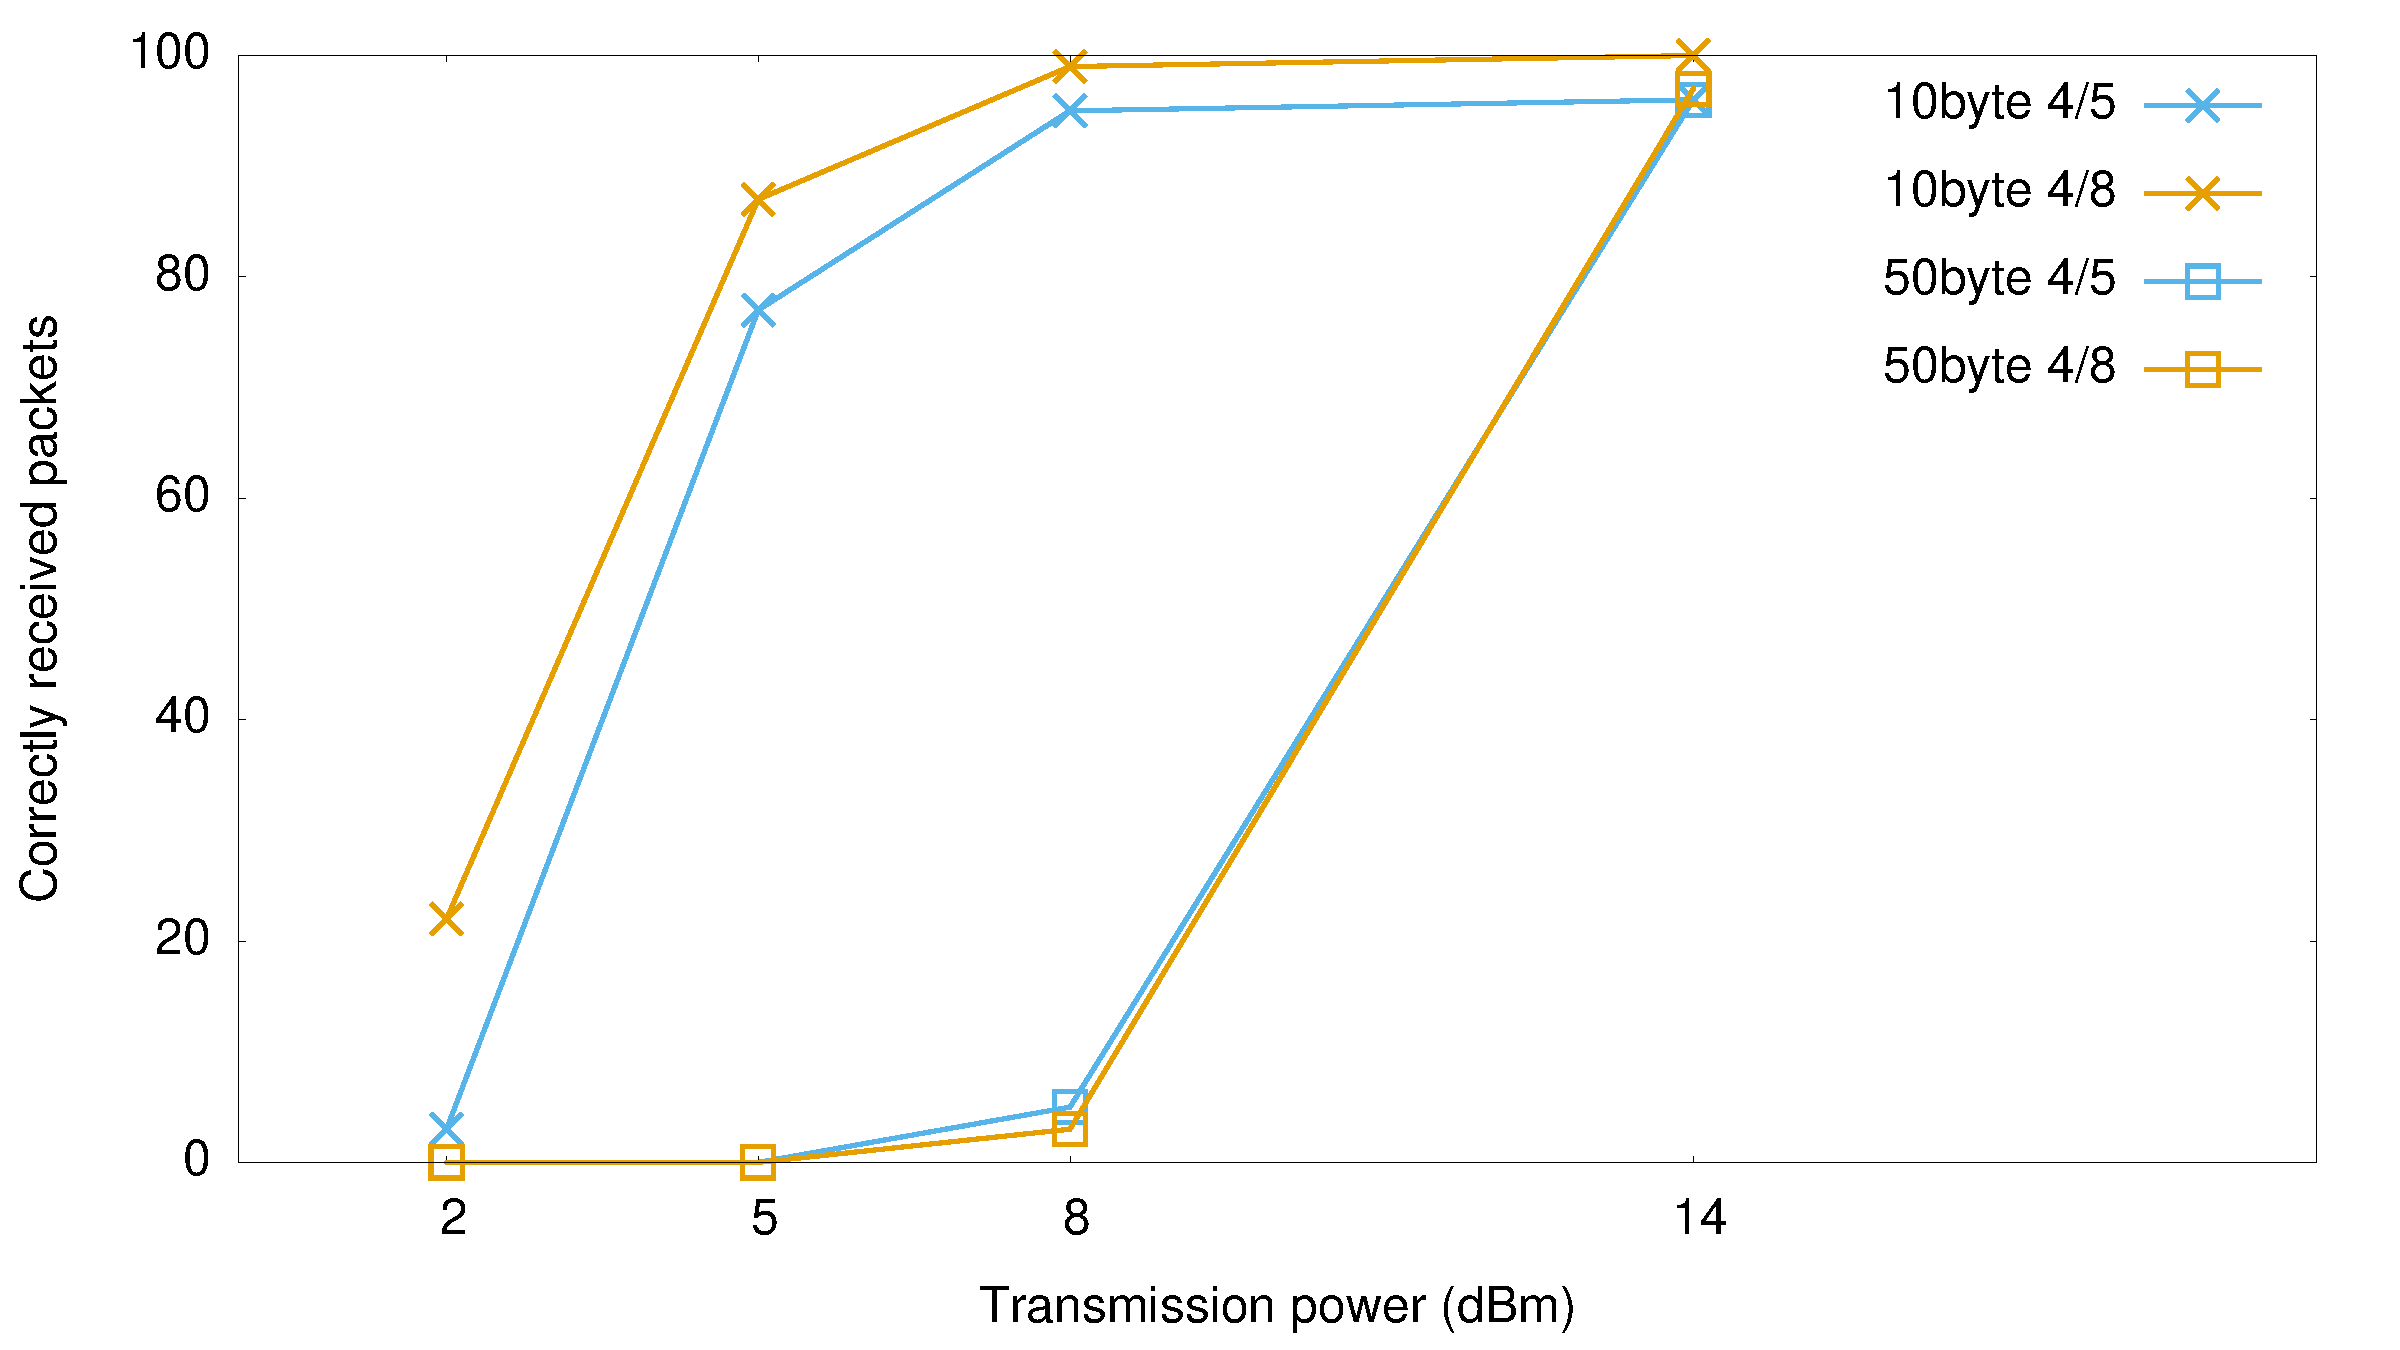
\includegraphics[width=\textwidth]{img/test/urban/sf8}
\caption{Results of urban experiments at SF 8}
\label{fig:sf8urban}
\end{figure}

\begin{figure}[]
\centering
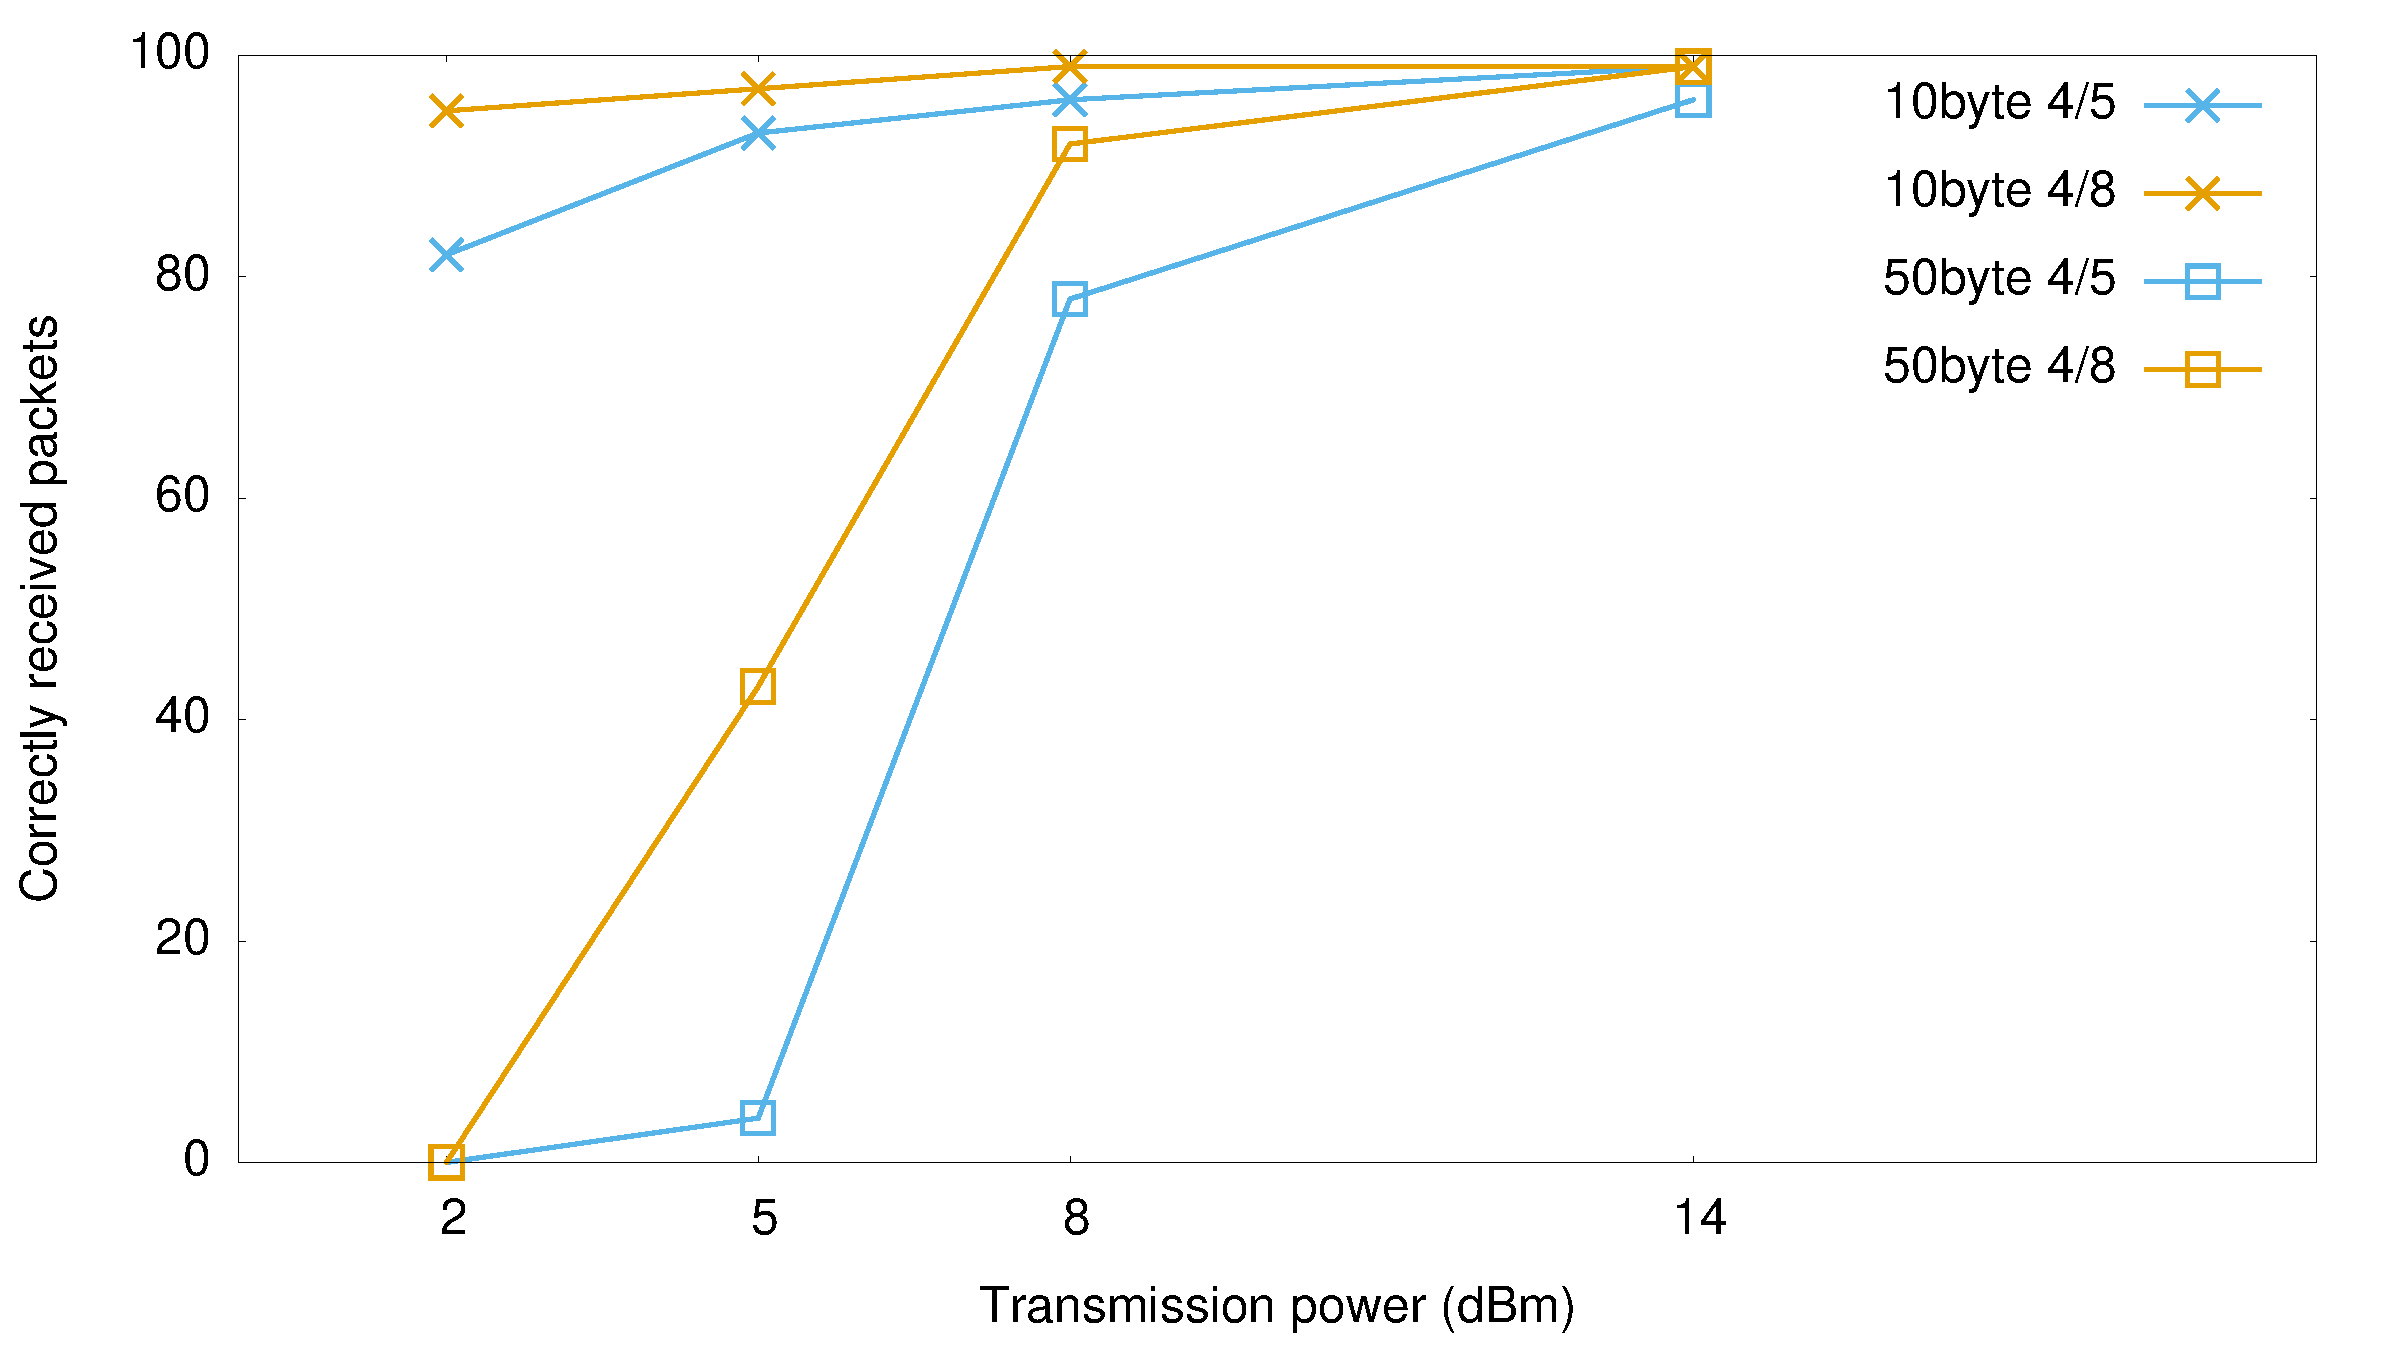
\includegraphics[width=\textwidth]{img/test/urban/sf9}
\caption{Results of urban experiments at SF 9}
\label{fig:sf9urban}
\end{figure}

\begin{figure}[]
\centering
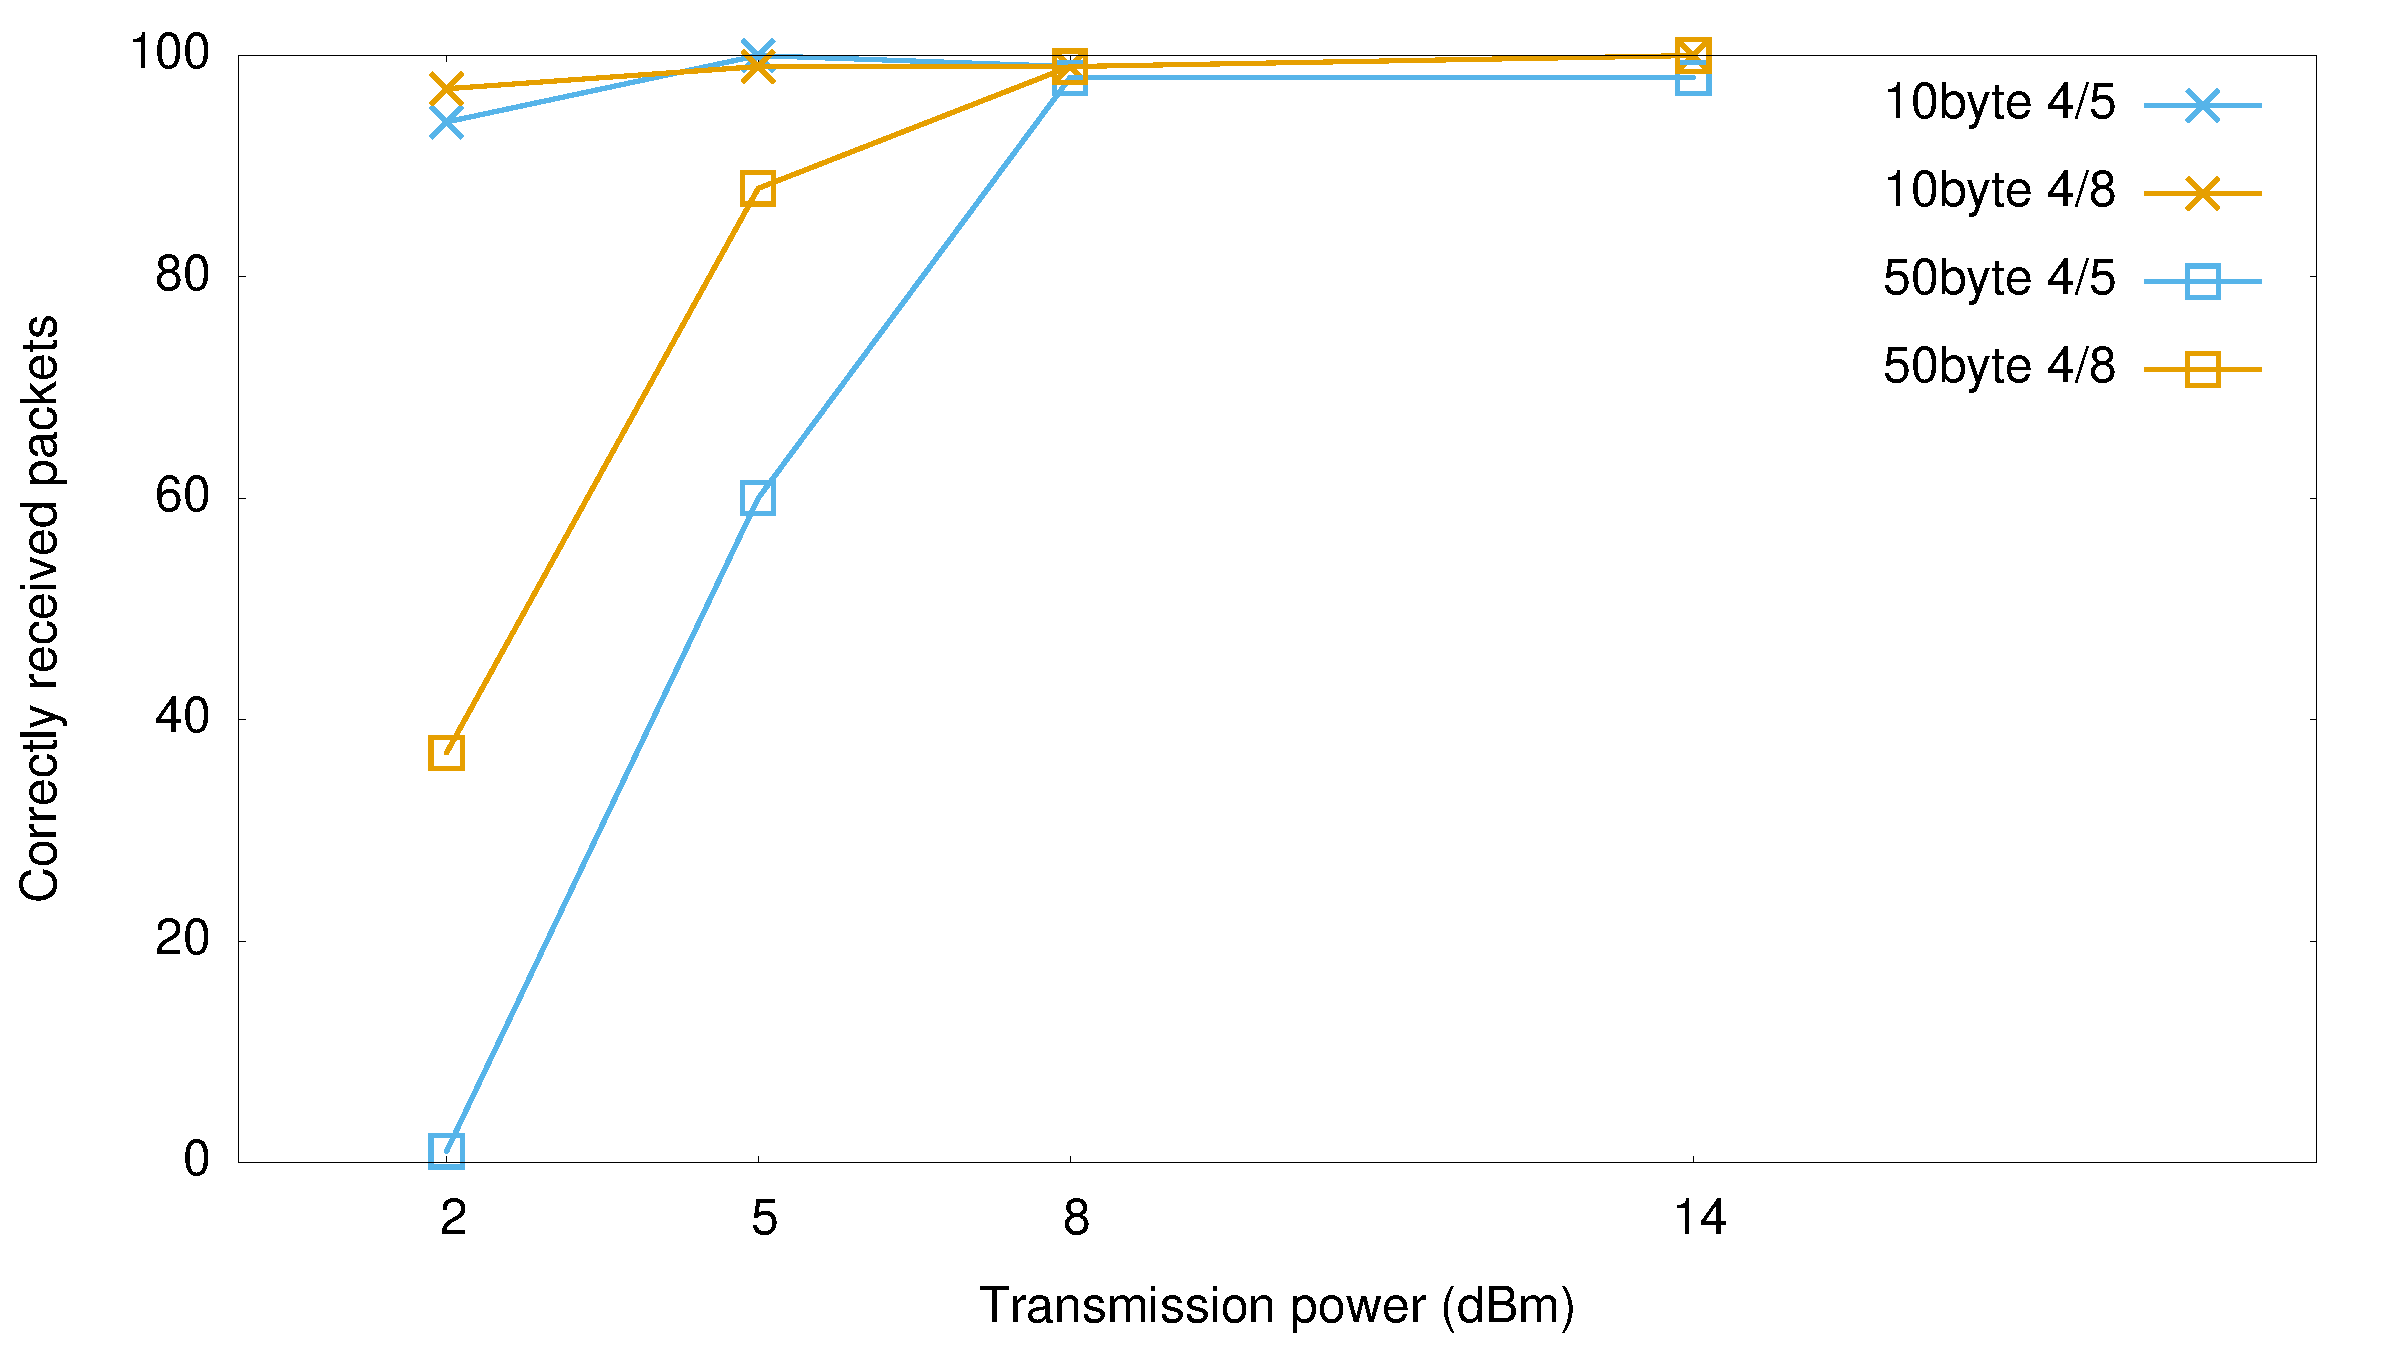
\includegraphics[width=\textwidth]{img/test/urban/sf10}
\caption{Results of urban experiments at SF 10}
\label{fig:sf10urban}
\end{figure}

\begin{figure}[]
\centering
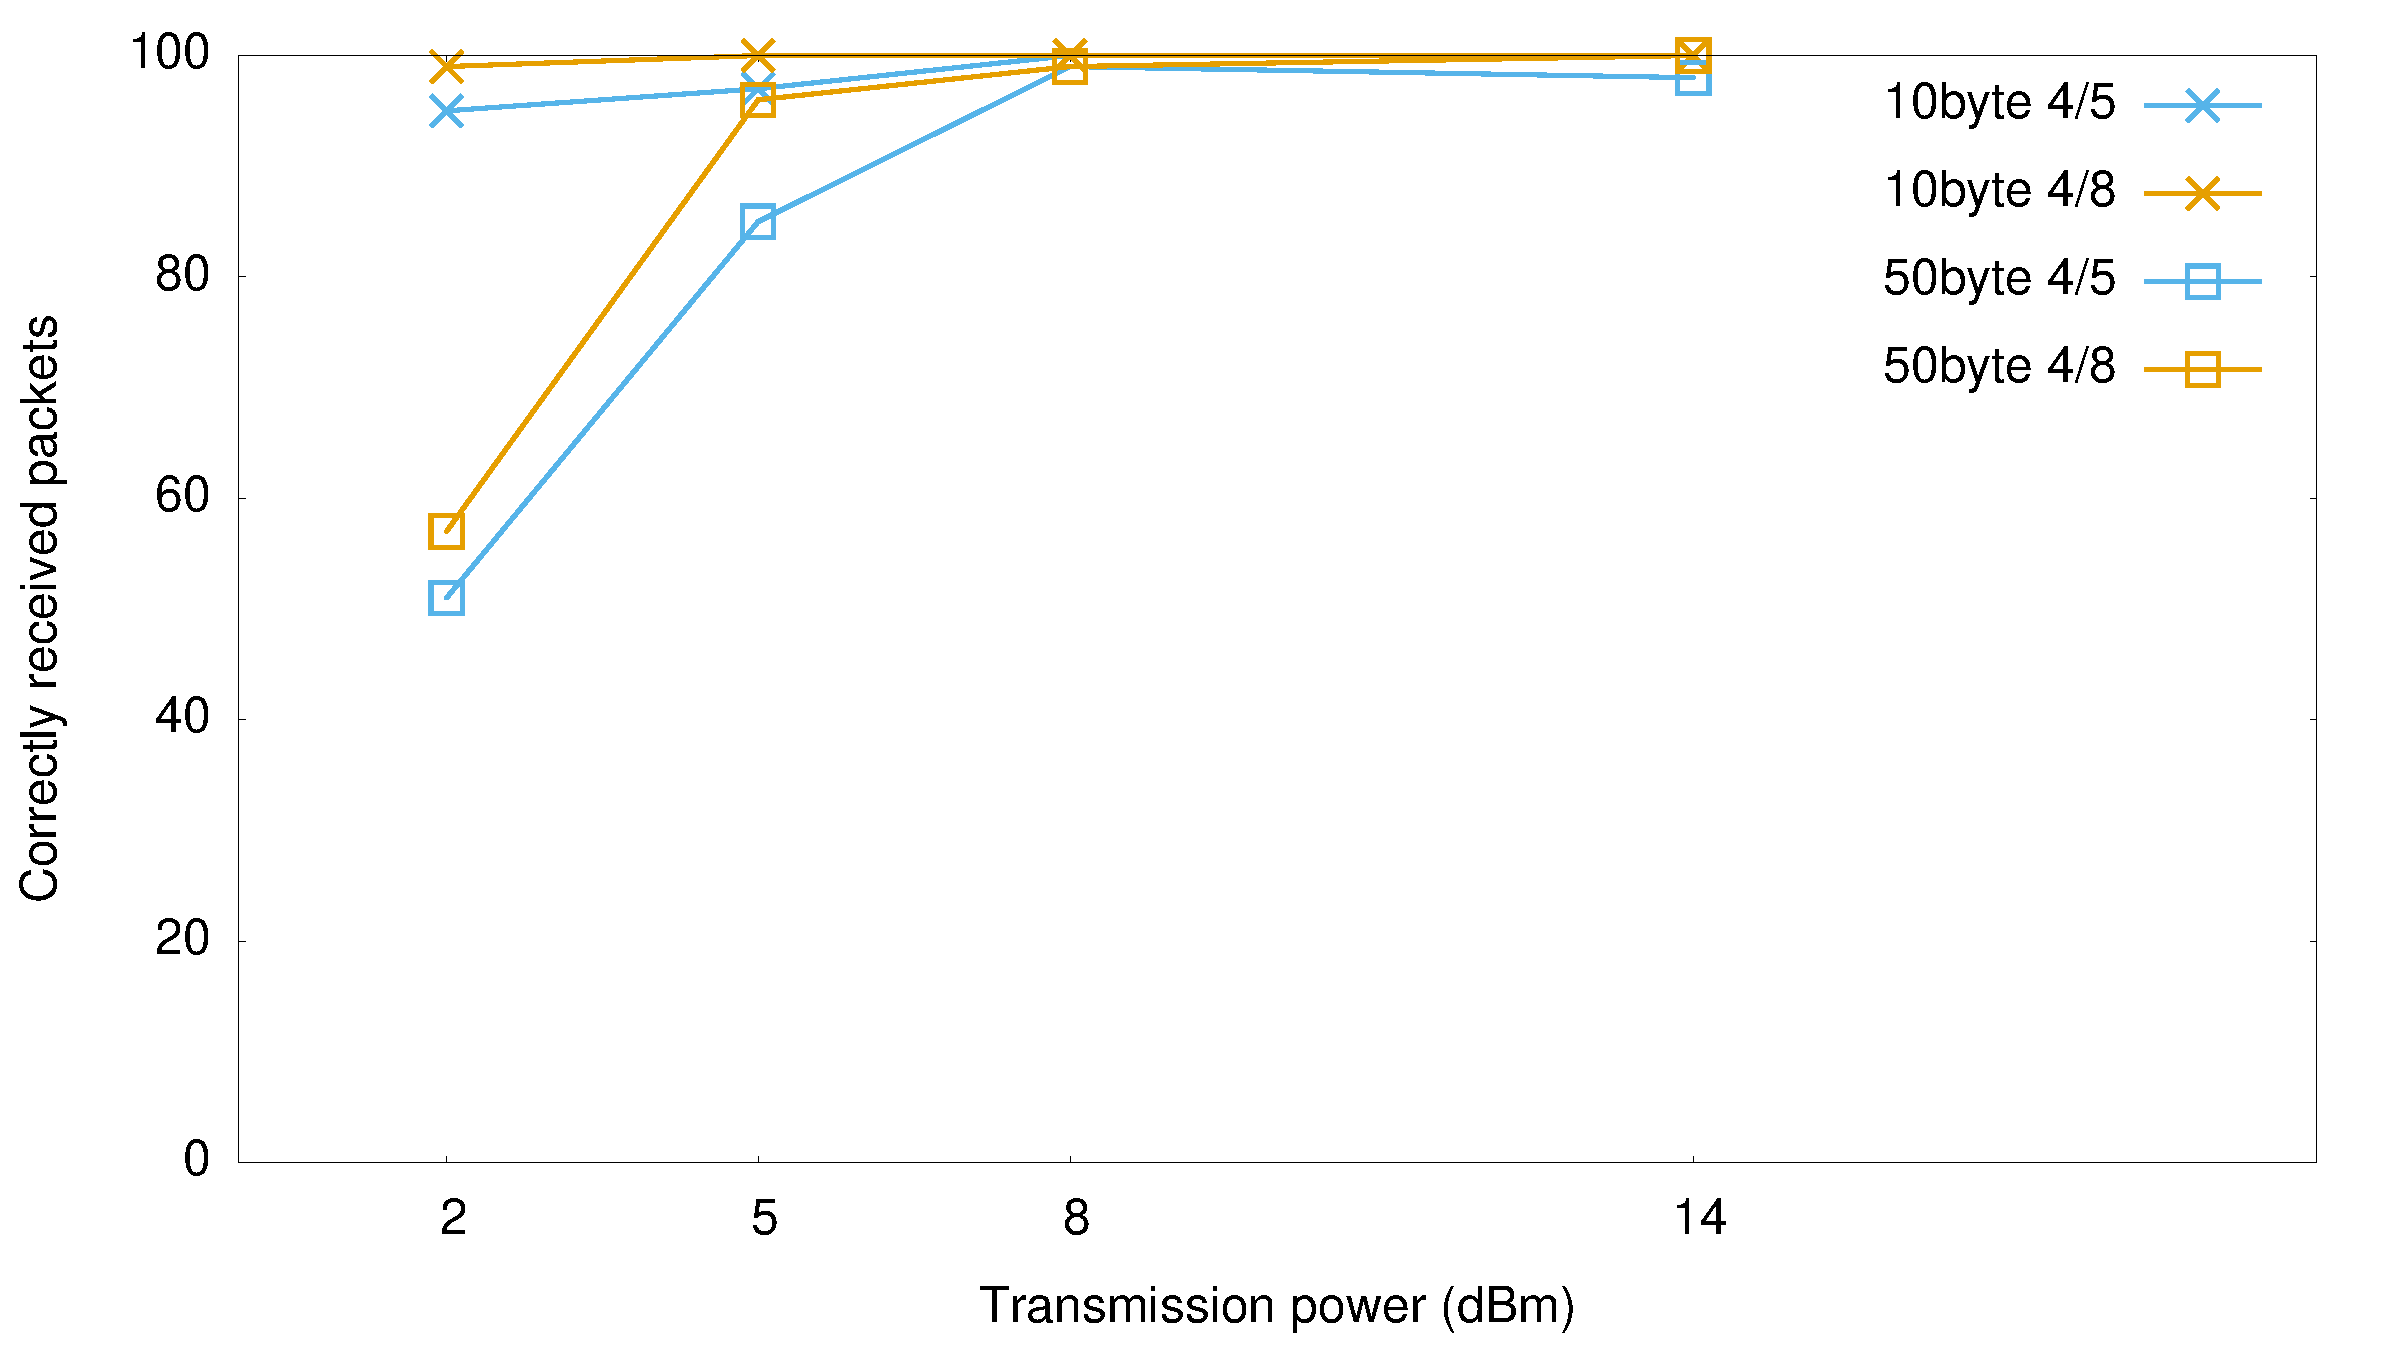
\includegraphics[width=\textwidth]{img/test/urban/sf11}
\caption{Results of urban experiments at SF 11}
\label{fig:sf11urban}
\end{figure}

\begin{figure}[]
\centering
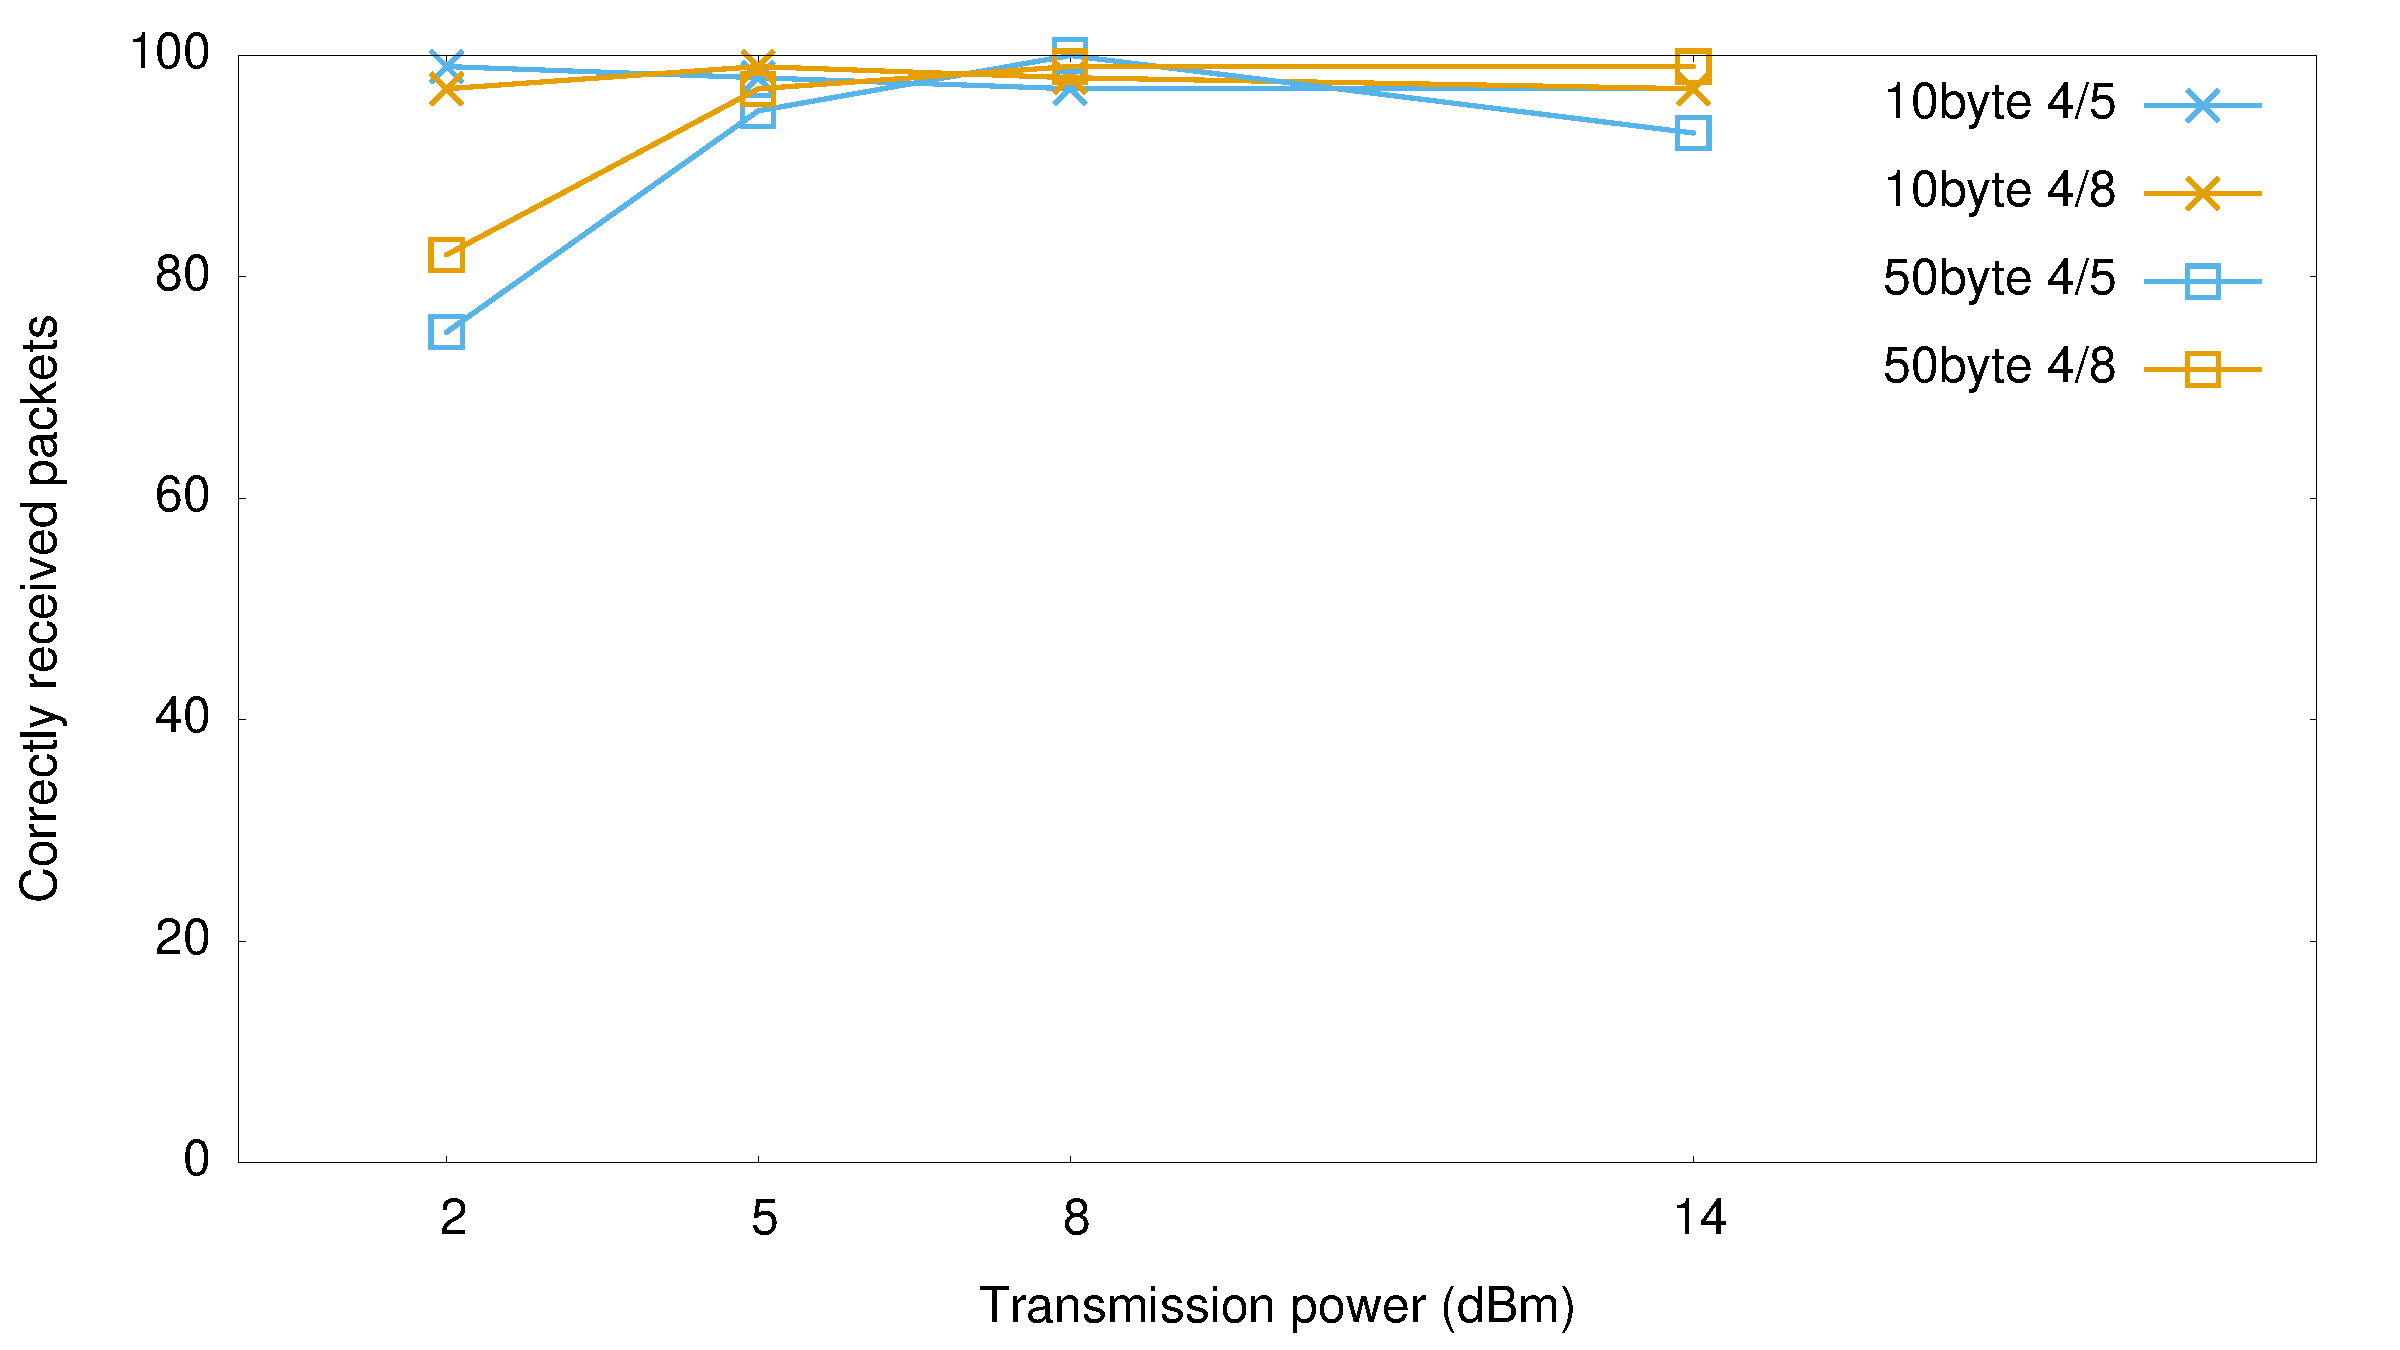
\includegraphics[width=\textwidth]{img/test/urban/sf12}
\caption{Results of urban experiments at SF 12}
\label{fig:sf12urban}
\end{figure}

\begin{figure}[]
\centering
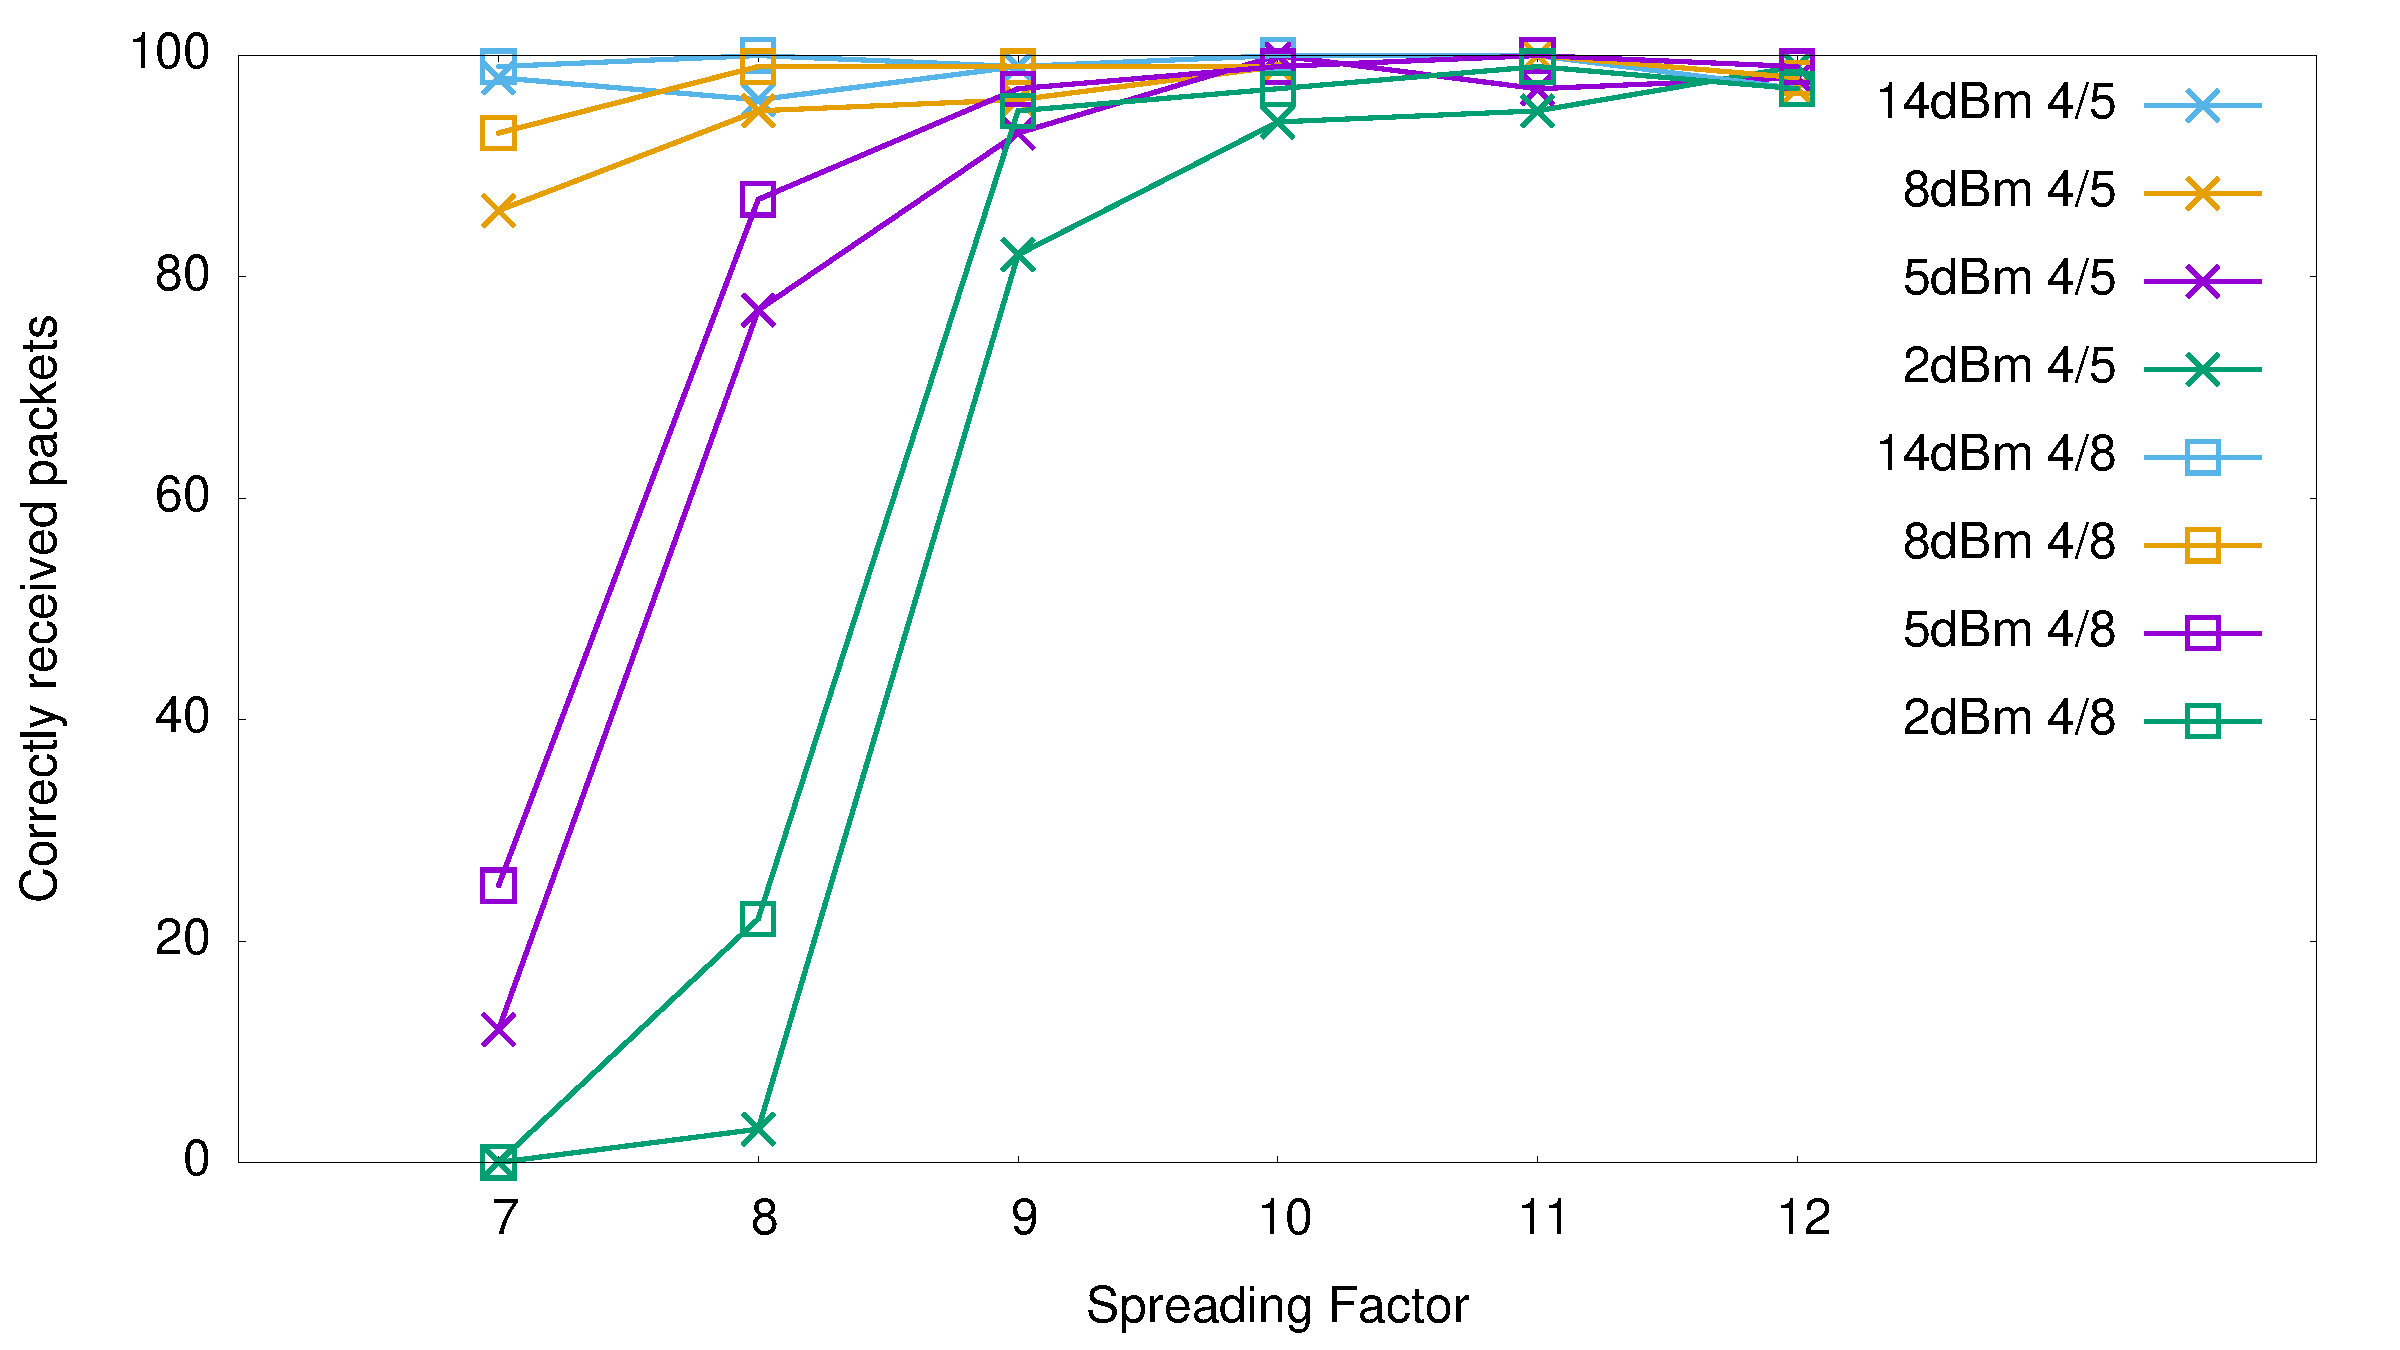
\includegraphics[width=\textwidth]{img/test/urban/len0}
\caption{Results of urban experiments with payload of 10 bytes}
\label{fig:len10urban}
\end{figure}

\begin{figure}[]
\centering
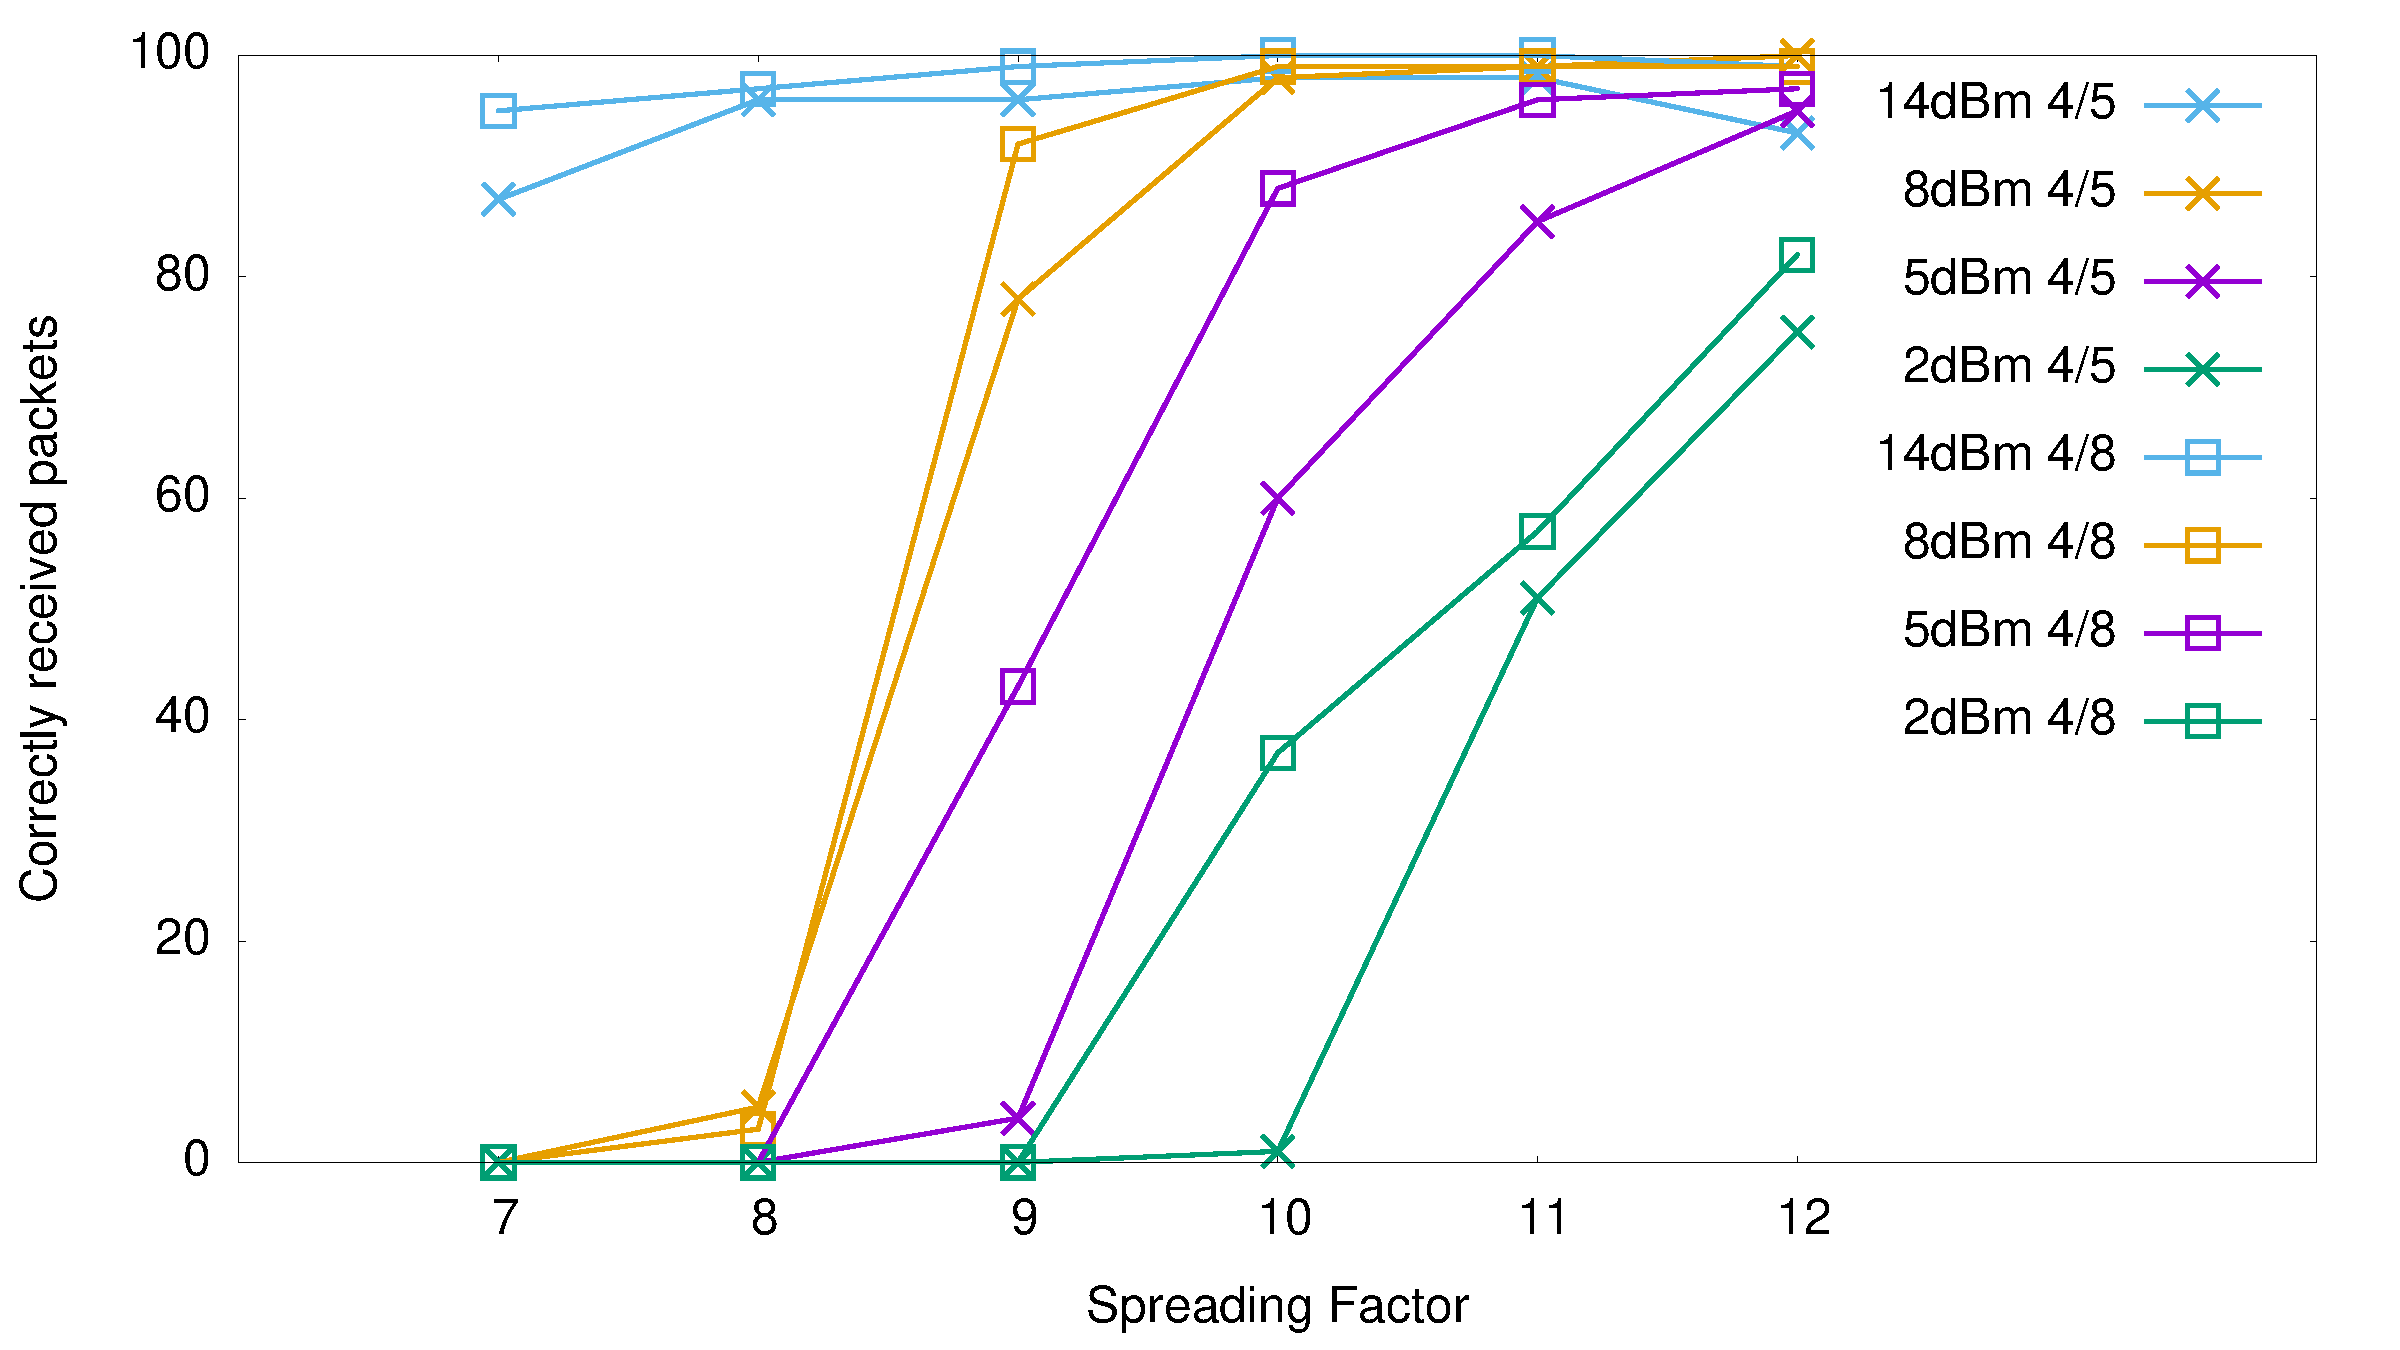
\includegraphics[width=\textwidth]{img/test/urban/len1}
\caption{Results of urban experiments with payload of 50 bytes}
\label{fig:len50urban}
\end{figure}







